\documentclass[12pt]{article}

\usepackage[utf8]{inputenc}
\usepackage{amsmath, amssymb, amsthm}
\usepackage{geometry}
\usepackage{setspace}
\usepackage{tikz}
\usetikzlibrary{positioning}
\usepackage{subcaption}
\usepackage{graphicx}
\usepackage{enumitem}
\usepackage{hyperref}
\usepackage{longtable}
\usepackage{booktabs}
\usepackage{bbm}
\usepackage{tikz-cd}
\usepackage{soul}
\sethlcolor{yellow} % Sets the highlight color
\usetikzlibrary{arrows.meta, positioning}
\usetikzlibrary{arrows.meta,calc,decorations.pathreplacing}

% -------------------------------------------------
% Color + framed boxes
% -------------------------------------------------
\usepackage{xcolor}
\definecolor{mygreen}{RGB}{0,140,0}
\definecolor{myblue}{RGB}{0,80,180}
\definecolor{myred}{RGB}{180,0,0}

\setlength{\fboxsep}{8pt}
\setlength{\fboxrule}{1.2pt}

\newcommand{\redbox}[1]{%
  \noindent\begingroup
  \setlength{\fboxsep}{8pt}%
  \setlength{\fboxrule}{1.2pt}%
  \fcolorbox{myred}{white}{%
    \parbox{\dimexpr\textwidth-2\fboxsep-2\fboxrule\relax}{\color{black}#1}%
  }%
  \endgroup
}

\newcommand{\bluebox}[1]{%
  \noindent\begingroup
  \setlength{\fboxsep}{8pt}%
  \setlength{\fboxrule}{1.2pt}%
  \fcolorbox{myblue}{white}{%
    \parbox{\dimexpr\textwidth-2\fboxsep-2\fboxrule\relax}{\color{black}#1}%
  }%
  \endgroup
}

\geometry{margin=1in}
\setstretch{1.5}

\DeclareMathOperator{\Var}{Var}

\newtheorem{assumption}{Assumption}
\newtheorem{lemma}{Lemma}
\theoremstyle{remark}
\newtheorem{remark}{Remark}
\newtheorem{example}{Example}
\theoremstyle{definition}
\newtheorem{corollary}{Corollary}
\newtheorem{definition}{Definition}
\newcommand{\E}{\mathbb{E}}

\def\EE{\mathbb{E}}
\def\PP{\mathbb{P}}
\def\RR{\mathbb{R}}

\title{}

\begin{document}
\maketitle

\subsection*{Subspaces}
\hfill \break  $~\!\!$ \dotfill \medskip \\

\redbox{
\textbf{Subspace Test.} Let $W \subseteq V$ where $V$ is a vector space over a field $\mathbb{F}$.

Then $W$ is a subspace of $V$ if and only if:
\begin{align*}
\forall x,y \in W,\; x+y \in W, \\
\forall a \in \mathbb{F},\; \forall x \in W,\; ax \in W.
\end{align*}
}

\medskip

\bluebox{
\textbf{Commentary:} These two conditions automatically imply:
\begin{itemize}[leftmargin=1.5em]
    \item $0 \in W$ (take $a=0$),
    \item closure under subtraction,
    \item all vector space axioms inherited from $V$.
\end{itemize}

So this is the minimal test for checking subspaces in practice.
}

\medskip
\hrule
\medskip

\subsection*{Linear Transformations}
\hfill \break  $~\!\!$ \dotfill \medskip \\

\redbox{
A map $T : V \to W$ (vector spaces over $\mathbb{F}$) is \textbf{linear} if:
\begin{align*}
T(x+y) &= T(x) + T(y), \\
T(ax) &= aT(x).
\end{align*}
}

\medskip

\bluebox{
\textbf{Commentary:} Linear maps preserve the vector space structure. In particular:
\[
T(0)=0,\quad T(x-y)=T(x)-T(y).
\]
Also, the image $T(V)$ is always a subspace of $W$.
}

\medskip
\hrule
\medskip

\subsection*{Bases and Coordinate Representation}
\hfill \break  $~\!\!$ \dotfill \medskip \\

\redbox{
Let $B=\{x_1,\dots,x_n\}$ be a basis of $V$. Then:

\begin{enumerate}[leftmargin=1.5em]
    \item $\text{span}\{x_1,\dots,x_n\}=V$
    \item $\{x_1,\dots,x_n\}$ is linearly independent
\end{enumerate}

Equivalently, every $x \in V$ can be written uniquely as
\begin{align*}
x = a_1 x_1 + \cdots + a_n x_n.
\end{align*}
}

\medskip

\bluebox{
\textbf{Commentary:} The key word is \textbf{uniquely}.

This allows us to define coordinates (coefficients of $x$ in the basis $B$):
\[
[x]_B = (a_1,\dots,a_n) \in \mathbb{F}^n.
\]

Thus choosing a basis turns an abstract vector space into $\mathbb{F}^n$.
}

\medskip
\hrule
\medskip

\subsection*{Coordinate Isomorphism}
\hfill \break  $~\!\!$ \dotfill \medskip \\

\redbox{
Define
\begin{align*}
[\cdot]_B : V \to \mathbb{F}^n, \quad x \mapsto [x]_B.
\end{align*}

Then this map is a linear isomorphism.
}

\medskip

\bluebox{
\textbf{Commentary:}
\begin{itemize}[leftmargin=1.5em]
    \item Linearity follows from linearity of coordinates:
    \[
    [x+y]_B = [x]_B + [y]_B,\quad [ax]_B = a[x]_B.
    \]
    \item Injective: unique representation
    \item Surjective: every vector in $\mathbb{F}^n$ corresponds to some $x$
\end{itemize}

So all finite-dimensional vector spaces of dimension $n$ are essentially $\mathbb{F}^n$.
}

\medskip
\hrule
\medskip

\subsection*{Matrix Representation of a Linear Map}
\hfill \break  $~\!\!$ \dotfill \medskip \\

\redbox{
Let $T: V \to W$ be linear, with bases $B$ for $V$ and $C$ for $W$.

Then there exists a matrix $[T]_{C \leftarrow B}$ such that
\begin{align*}
[T(x)]_C = [T]_{C \leftarrow B} \,[x]_B.
\end{align*}
}

\medskip

\bluebox{
\textbf{Commentary:}
\begin{itemize}[leftmargin=1.5em]
    \item The matrix is constructed by applying $T$ to basis vectors:
    \[
    [T(x_j)]_C = \text{column } j.
    \]
    \item This converts abstract linear maps into matrix multiplication.
\end{itemize}

So linear algebra = matrix algebra once a basis is fixed.
}

\medskip
\hrule
\medskip

\subsection*{Change of Basis}
\hfill \break  $~\!\!$ \dotfill \medskip \\

\redbox{
Let $B,B'$ be two bases of $V$. Then there exists an invertible matrix $Q$ such that
\begin{align*}
[x]_{B'} = Q [x]_B.
\end{align*}

$Q$ is called the \textbf{change of coordinate matrix} from $B$ to $B'$.
}

\medskip

\bluebox{
\textbf{Commentary:}
\begin{itemize}[leftmargin=1.5em]
    \item Columns of $Q$ are the coordinates of the old basis vectors in the new basis.
    \item $Q$ is always invertible.
    \item $Q^{-1}$ converts back.
\end{itemize}

So coordinates depend on basis, but the underlying vector does not.
}

\medskip
\hrule
\medskip

\subsection*{Change of Matrix Representation}
\hfill \break  $~\!\!$ \dotfill \medskip \\

\redbox{
Let $T: V \to V$ and let $B,B'$ be two bases.

If $Q$ is the change-of-basis matrix, then
\begin{align*}
[T]_{B'} = Q [T]_B Q^{-1}.
\end{align*}
}

\medskip

\bluebox{
\textbf{Commentary:}
This is called a \textbf{similarity transformation}.

It shows:
\begin{itemize}[leftmargin=1.5em]
    \item Different matrices can represent the same linear operator
    \item They are related by conjugation
    \item $T$ is the actual linear transformation between vector spaces.
    \item $[T]_B$ is the matrix that represents $T$ once basis $B$ is chosen.
\end{itemize}

This is the foundation of:
\begin{itemize}[leftmargin=1.5em]
    \item diagonalization
    \item eigenvalues
    \item canonical forms
\end{itemize}
}

\medskip
\hrule
\medskip

\subsection*{Big Picture Diagram}
\hfill \break  $~\!\!$ \dotfill \medskip \\

\bluebox{
\textbf{Conceptual Summary:}

\[
\begin{array}{ccc}
V & \xrightarrow{T} & V \\
\downarrow [\cdot]_B & & \downarrow [\cdot]_B \\
\mathbb{F}^n & \xrightarrow{[T]_B} & \mathbb{F}^n
\end{array}
\]

Changing basis inserts $Q$:

\[
[T]_{B'} = Q [T]_B Q^{-1}.
\]

So:
\begin{itemize}[leftmargin=1.5em]
    \item Abstract map $\leftrightarrow$ matrix
    \item Basis choice $\leftrightarrow$ coordinate system
    \item Change of basis $\leftrightarrow$ similarity transform
\end{itemize}
}

\bluebox{
$V$ and $\mathbb{F}^n$ are usually \textbf{isomorphic}, not \textbf{equal}.

When we say $V$ is an $n$-dimensional vector space over $F$, that means $V$ has the same vector-space structure as $F^n$, but its elements need not already be $n$-tuples.

So the distinction is: $V \cong F^n$ but usually not $V = F^n$. 

A vector space is not determined just by ``field $F$ + dimension $n$'' as a set. Many different-looking objects can all be $n$-dimensional vector spaces over $F$.

Examples of $2$-dimensional vector spaces over $\mathbb{R}$:

- $\mathbb{R}^2$
- the space of polynomials of degree $\le 1$, $P_1(\mathbb{R})$
- the space of $2\times 2$ diagonal matrices
- any plane through the origin in $\mathbb{R}^3$

All of these are $2$-dimensional over $\mathbb{R}$, so each is isomorphic to $\mathbb{R}^2$, but they are not the same set and their elements do not look the same.
}

\bluebox{
For instance, in $P_1(\mathbb{R})$, a vector looks like $a+bx$, not like $(a,b)$.

Once you choose an ordered basis, say $B=(1,x)$, then every polynomial $a+bx$ gets identified with its coordinate vector $[a+bx]_B=\begin{pmatrix} a \\ b \end{pmatrix}\in\mathbb{R}^2$.

That coordinate map is the isomorphism.

So the reason I distinguish $V$ and $F^n$ is:

- $V$ is the original abstract vector space
- $F^n$ is the coordinate model you get after choosing a basis

A basis gives a specific map $[\cdot]_B:V\to F^n$, and that map depends on the basis.

Without choosing a basis, there is no canonical way to say which vector in $V$ corresponds to which tuple in $F^n$.

That is why $V$ is not automatically $F^n$. It becomes identified with $F^n$ only after a basis is chosen.

A useful analogy: two sets can have the same number of elements without being literally the same set. Likewise, two vector spaces can have the same dimension over the same field without being literally the same vector space.

So the clean statement is:

\textbf{Every $n$-dimensional vector space over $F$ is isomorphic to $\mathbb{F}^n$, but not automatically equal to $F^n$.}

The only time you would write $V=F^n$ is when the vector space actually has already been defined to be $F^n$.
}

\subsection*{Vector Spaces and Subspaces}

Let $F$ be a field and let $V$ be a vector space over $F$.

A subset $W \subseteq V$ is called a \emph{subspace} if:
\begin{enumerate}
    \item $0 \in W$,
    \item $x,y \in W \Rightarrow x+y \in W$,
    \item $a \in F,\, x \in W \Rightarrow ax \in W$.
\end{enumerate}

\begin{center}
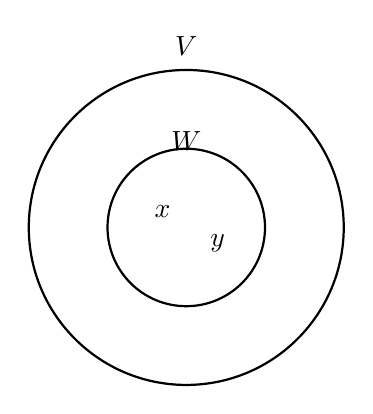
\begin{tikzpicture}
  \draw[thick] (0,0) circle (2);
  \draw[thick] (0,0) circle (1);
  \node at (0,2.3) {$V$};
  \node at (0,1.1) {$W$};
  \node at (-0.3,0.2) {$x$};
  \node at (0.4,-0.2) {$y$};
\end{tikzpicture}
\end{center}

\subsection*{Bases and Coordinates}

Let $V$ be an $n$--dimensional vector space over $F$.
An ordered set
\[
\mathcal{B} = \{x_1,\dots,x_n\}
\]
is a \emph{basis} of $V$ if:
\begin{enumerate}
    \item $\operatorname{span}\{x_1,\dots,x_n\} = V$,
    \item $\{x_1,\dots,x_n\}$ is linearly independent.
\end{enumerate}

Every $x \in V$ can be written uniquely as

\[
x = a_1 x_1 + \cdots + a_n x_n,
\qquad a_i \in F.
\]

Define the coordinate vector of $x$ relative to $\mathcal{B}$ by

\[
[x]_{\mathcal{B}} =
\begin{bmatrix}
a_1 \\ \vdots \\ a_n
\end{bmatrix}
\in F^n.
\]

\subsection*{Coordinate Map Is an Isomorphism}

Define the map
\[
\Phi_{\mathcal{B}} : V \to F^n,
\qquad
\Phi_{\mathcal{B}}(x) = [x]_{\mathcal{B}}.
\]

Then $\Phi_{\mathcal{B}}$ is a linear isomorphism.

\begin{center}
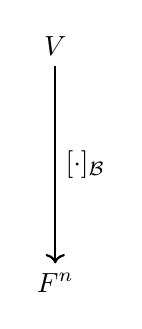
\begin{tikzpicture}[node distance=3cm]
\node (V) {$V$};
\node (Fn) [below of=V] {$F^n$};

\draw[->, thick] (V) -- node[right] {$[\cdot]_{\mathcal{B}}$} (Fn);
\end{tikzpicture}
\end{center}

Let $\mathcal{B}$ and $\mathcal{B}'$ be two ordered bases of $V$. Note that order matters because coordinates depend on it.



\subsection*{Change of Basis Matrix}

There exists an invertible matrix $Q \in F^{n \times n}$ such that
\[
[x]_{\mathcal{B}} = Q [x]_{\mathcal{B}'}.
\]

The matrix $Q$ is called the \emph{change of coordinate matrix}
from $\mathcal{B}'$ to $\mathcal{B}$.

\begin{center}
\begin{tikzcd}
V \arrow[d, "{[\cdot]_{\mathcal{B}'}}"'] \arrow[dr, "{[\cdot]_{\mathcal{B}}}"] & \\
F^n \arrow[r, "Q"] & F^n
\end{tikzcd}
\end{center}

\subsection*{Matrix Representation of Linear Transformations}

Let $T: V \to V$ be linear and let $\mathcal{B}$ be a basis of $V$.

There exists a unique matrix $[T]_{\mathcal{B}} \in F^{n \times n}$ such that
\[
[T(x)]_{\mathcal{B}} = [T]_{\mathcal{B}} [x]_{\mathcal{B}}
\]
for all $x \in V$.

\begin{center}
\begin{tikzcd}[column sep=huge, row sep=huge]
V \arrow[r, "T"]
  \arrow[d, shift right=2pt, "{[\cdot]_{\mathcal{B}'}}"']
& V \arrow[d, shift left=2pt, "{[\cdot]_{\mathcal{B}'}}"] \\
F^n \arrow[r, "{[T]_{\mathcal{B}'}}"]
    \arrow[u, shift right=2pt, "Q"']
& F^n \arrow[u, shift left=2pt, "Q"]
\end{tikzcd}
\end{center}

The key insight the diagram captures is that the square commutes — there are two paths from $V$ (top-left) to $\mathbb{F}^n$ (bottom-right), and they always give the same answer. 

\textbf{Route 1:} Apply $T$ first (stay in abstract $V$), then coordinatize via $[\cdot]_{\mathcal{B}}$.

\textbf{Route 2:} Coordinatize $x$ first to get $[x]_{\mathcal{B}} \in F^n$, then multiply by the matrix $[T]_{\mathcal{B}}$.

The theorem says these are identical, which is exactly what $    [T(x)]_{\mathcal{B}} = [T]_{\mathcal{B}}\, [x]_{\mathcal{B}}$ asserts. The matrix $[T]_{\mathcal{B}}$ exists precisely to make this square commute---it translates the abstract linear map $T$ into concrete matrix multiplication in coordinate space $F^n$.

Let $\mathcal{B}, \mathcal{B}'$ be two bases and let $Q$ be the change-of-basis matrix.


\subsection*{Change of Basis and Similar Matrices}

Let $T : V \to V$ be a linear map, and let $\mathcal{B}$ and $\mathcal{B}'$ be two bases of $V$.
Let $Q$ be the change-of-basis matrix from $\mathcal{B}'$ to $\mathcal{B}$, so that
$[x]_{\mathcal{B}} = Q\,[x]_{\mathcal{B}'}$ for all $x \in V$.

\medskip
The matrix representations of $T$ in the two bases satisfy
\[
    [T]_{\mathcal{B}} \;=\; Q\,[T]_{\mathcal{B}'}\,Q^{-1}.
\]
Thus, different matrix representations of the same linear operator are \emph{similar matrices}.

\medskip
\noindent\textbf{Commutative diagram.}
The identity is witnessed by the following commutative square,
in which both routes from $V$ (top-left) to $F^n$ (bottom-right) agree.

Original diagram from lecture:\\

\begin{center}
\begin{tikzcd}[column sep=8em, row sep=6em]
F^n \arrow[r, "{[T]_{\mathcal{B}'}}"] 
    \arrow[d, shift right=2ex, "Q"'] 
& F^n \arrow[d, shift left=2ex, "Q"] \\
F^n \arrow[r, "{[T]_{\mathcal{B}}}"] 
    \arrow[u, shift right=2ex, "Q^{-1}"] 
& F^n \arrow[u, shift left=2ex, "Q^{-1}"']
\end{tikzcd}
\end{center}



\noindent The key insight is that the diagram is \emph{not} showing two
separate maps per side. Rather, it is showing one isomorphism per side
with both the forward and backward directions labeled simultaneously.
Specifical

More detailed version:\\
\begin{center}
\begin{tikzcd}[column sep=huge, row sep=large]
V \arrow[r, "T"] \arrow[d, "{[\cdot]_{\mathcal{B}'}}"']
& V \arrow[d, "{[\cdot]_{\mathcal{B}'}}"] \\
F^n \arrow[r, "{[T]_{\mathcal{B}'}}"] \arrow[d, "Q"']
& F^n \arrow[d, "Q"] \\
F^n \arrow[r, "{[T]_{\mathcal{B}}}"] \arrow[u, bend right=40, "Q^{-1}"']
& F^n
\end{tikzcd}
\end{center}

\medskip
\noindent\textbf{Step-by-step verification.}
Fix $x \in V$.

\begin{enumerate}
    \item \textbf{Route 1 (top, then right):}
    Apply $T$ to get $T(x) \in V$, then coordinatize in $\mathcal{B}'$:
    \[
        x \;\xrightarrow{\;T\;}\; T(x)
          \;\xrightarrow{\;[\cdot]_{\mathcal{B}'}\;}\;
          [T(x)]_{\mathcal{B}'} \;=\; [T]_{\mathcal{B}'}\,[x]_{\mathcal{B}'}
          \;\in\; F^n.
    \]

    \item \textbf{Route 2 (left, then bottom):}
    Convert $x$ from $\mathcal{B}$-coordinates to $\mathcal{B}'$-coordinates via $Q^{-1}$,
    then apply $[T]_{\mathcal{B}'}$:
    \[
        x \;\xrightarrow{\;Q^{-1} \circ [\cdot]_{\mathcal{B}}\;}\;
          Q^{-1}[x]_{\mathcal{B}} \;=\; [x]_{\mathcal{B}'}
          \;\xrightarrow{\;[T]_{\mathcal{B}'}\;}\;
          [T]_{\mathcal{B}'}\,Q^{-1}[x]_{\mathcal{B}}
          \;\in\; F^n.
    \]

    \item \textbf{Commutativity:}
    Both routes produce the same element of $F^n$, so for all $x \in V$:
    \[
        [T]_{\mathcal{B}'}\,[x]_{\mathcal{B}'} \;=\; [T]_{\mathcal{B}'}\,Q^{-1}[x]_{\mathcal{B}}.
    \]
    Since $[x]_{\mathcal{B}'} = Q^{-1}[x]_{\mathcal{B}}$, this is consistent.
    Now recall that by definition of $[T]_{\mathcal{B}}$:
    \[
        [T(x)]_{\mathcal{B}} \;=\; [T]_{\mathcal{B}}\,[x]_{\mathcal{B}}.
    \]
    Expressing $[T(x)]_{\mathcal{B}} = Q\,[T(x)]_{\mathcal{B}'}
    = Q\,[T]_{\mathcal{B}'}\,Q^{-1}[x]_{\mathcal{B}}$
    and equating with $[T]_{\mathcal{B}}\,[x]_{\mathcal{B}}$ gives,
    since this holds for all $x$:
    \[
        \boxed{[T]_{\mathcal{B}} \;=\; Q\,[T]_{\mathcal{B}'}\,Q^{-1}.}
    \]

    \item \textbf{Geometric reading of $Q\,[T]_{\mathcal{B}'}\,Q^{-1}$:}
    Reading right to left, $Q^{-1}$ converts input coordinates from $\mathcal{B}$
    to $\mathcal{B}'$ (left arrow, going down); $[T]_{\mathcal{B}'}$ applies the
    transformation in the $\mathcal{B}'$-coordinate system (bottom arrow, going right);
    and $Q$ converts the result back from $\mathcal{B}'$-coordinates to
    $\mathcal{B}$-coordinates. The conjugation $Q\,(\cdot)\,Q^{-1}$ is a round-trip
    change of coordinates sandwiching the computation.
\end{enumerate}

\noindent\textbf{Where does $[x]_{\mathcal{B}'}$ come from?}

\medskip
The change-of-basis matrix $Q$ is defined by the relation
\[
    [x]_{\mathcal{B}} \;=\; Q\,[x]_{\mathcal{B}'}
    \qquad \text{for all } x \in V.
\]
Multiplying both sides on the left by $Q^{-1}$ gives immediately
\[
    Q^{-1}[x]_{\mathcal{B}} \;=\; [x]_{\mathcal{B}'}.
\]
This is the entire justification---no separate computation is needed.

\medskip
The left vertical arrow in the commutative diagram is labeled
$Q^{-1} \circ [\cdot]_{\mathcal{B}}$, which decomposes into two steps:
\begin{enumerate}
    \item Apply $[\cdot]_{\mathcal{B}}$: extract the $\mathcal{B}$-coordinates
    of $x$, producing $[x]_{\mathcal{B}} \in F^n$.
    \item Multiply by $Q^{-1}$: convert from $\mathcal{B}$-coordinates to
    $\mathcal{B}'$-coordinates, producing $Q^{-1}[x]_{\mathcal{B}} = [x]_{\mathcal{B}'} \in F^n$.
\end{enumerate}
The composition $Q^{-1} \circ [\cdot]_{\mathcal{B}}$ therefore sends $x \mapsto [x]_{\mathcal{B}'}$,
which is exactly the coordinatization map $[\cdot]_{\mathcal{B}'}$ applied directly.


\noindent\textbf{Reconciliation with the original diagram.}

The vertical arrows in the diagram are isomorphisms, and the diagram
labels both directions simultaneously. Specifically, the
coordinatization map $[\cdot]_{\mathcal{B}'} : V \to F^n$ is an
isomorphism whose inverse is $Q : F^n \to V$, since $Q$ reconstructs
an abstract vector from its $\mathcal{B}'$-coordinates:
\[
    Q\,[x]_{\mathcal{B}'} \;=\; x
    \qquad \Longleftrightarrow \qquad
    [\cdot]_{\mathcal{B}'} \;=\; Q^{-1}.
\]
Thus on each vertical side, the two labels refer to the \emph{same}
isomorphism viewed in opposite directions:
\begin{itemize}
    \item Left side going down: $[\cdot]_{\mathcal{B}'} = Q^{-1}$
    \item Left side going up: $Q^{-1}$ --- same map, inverse direction shown for clarity
    \item Right side going down: $[\cdot]_{\mathcal{B}'} = Q^{-1}$
    \item Right side going up: $Q$ --- the inverse, reconstructing $x \in V$
\end{itemize}
The commutative square then reads: starting from $x \in V$ in the
top-left, both routes to $F^n$ in the bottom-right agree:
\begin{align*}
\text{Route 1 (top then right):} &\quad
    x \xrightarrow{T} T(x) \xrightarrow{[\cdot]_{\mathcal{B}'}} [T(x)]_{\mathcal{B}'} \\
\text{Route 2 (left then bottom):} &\quad
    x \xrightarrow{Q^{-1}} [x]_{\mathcal{B}'} \xrightarrow{[T]_{\mathcal{B}'}} [T]_{\mathcal{B}'}[x]_{\mathcal{B}'}
\end{align*}
Commutativity gives $[T(x)]_{\mathcal{B}'} = [T]_{\mathcal{B}'}[x]_{\mathcal{B}'}$
for all $x \in V$, which is precisely the definition of $[T]_{\mathcal{B}'}$.
The relation $[T]_{\mathcal{B}} = Q[T]_{\mathcal{B}'}Q^{-1}$ then follows
by conjugating both sides by $Q$.


\subsection*{Sum and Direct Sum of Subspaces}

\redbox{
Let $W_1, W_2 \subseteq V$ be subspaces.

\[
W_1 + W_2 = \{x_1 + x_2 : x_1 \in W_1, x_2 \in W_2\}.
\]

Then $W_1 + W_2$ is a subspace and is the smallest subspace containing both.
}

\medskip

\bluebox{
Union $W_1 \cup W_2$ is generally NOT a subspace (fails closure).
Sum fixes this by enforcing closure.
}

\medskip
\hrule
\medskip

\redbox{
\textbf{Direct Sum.}
\[
V = W_1 \oplus W_2
\]
iff every $v \in V$ can be written uniquely as
\[
v = x_1 + x_2,\quad x_1 \in W_1,\; x_2 \in W_2.
\]
}

\medskip

\bluebox{
Equivalent condition:
\[
W_1 \cap W_2 = \{0\}.
\]

Uniqueness proof (missing in notes):

If
\[
x_1 + x_2 = y_1 + y_2,
\]
then
\[
x_1 - y_1 = y_2 - x_2 \in W_1 \cap W_2,
\]
so both sides are $0$, hence uniqueness.
}

\medskip
\hrule
\medskip

\subsection*{Rank--Nullity Theorem}
\hfill \break  $~\!\!$ \dotfill \medskip \\

\redbox{
\textbf{Theorem (Rank--Nullity).} Let $T: V \to W$ be a linear transformation. Then
\[
\dim(\ker T) + \dim(\operatorname{Im} T) = \dim(V).
\]
Equivalently, $\dim(\text{domain}) = \dim(\text{kernel}) + \dim(\text{image})$.
}

\medskip

\bluebox{
\textbf{Commentary:} This is one of the central theorems of linear algebra. It says the dimension of the domain splits into the ``lost'' dimensions (kernel) and the ``surviving'' dimensions (image). Also note:
\begin{itemize}[leftmargin=1.5em]
    \item The image of a subspace under a linear map is a subspace of the codomain.
    \item The preimage of a subspace under a linear map is a subspace of the domain.
\end{itemize}
}

\medskip
\hrule
\medskip

\subsection*{Basis as Direct Sum}
\hfill \break  $~\!\!$ \dotfill \medskip \\

\redbox{
$\{v_1, \dots, v_n\}$ is a basis for $V$ if and only if
\[
V = \operatorname{span}\{v_1\} \oplus \operatorname{span}\{v_2\} \oplus \cdots \oplus \operatorname{span}\{v_n\}.
\]
}

\medskip

\bluebox{
\textbf{Commentary:} A basis decomposes $V$ into a direct sum of $1$-dimensional subspaces. Each coordinate $a_i$ in $v = a_1 v_1 + \cdots + a_n v_n$ corresponds to the component in $\operatorname{span}\{v_i\}$, and the direct sum guarantees this decomposition is unique.

\textbf{Example:} In $\mathbb{R}^3$ with the standard basis $\{e_1, e_2, e_3\}$:
\[
\mathbb{R}^3 = \operatorname{span}\{e_1\} \oplus \operatorname{span}\{e_2\} \oplus \operatorname{span}\{e_3\}
\]
where each summand is one of the coordinate axes.
}

\medskip
\hrule
\medskip

%% ============================================================
%% COMPLEX NUMBERS (Feb 10 lecture)
%% ============================================================

\subsection*{The Complex Numbers}
\hfill \break  $~\!\!$ \dotfill \medskip \\

\redbox{
\textbf{Definition.} As a set,
\[
\mathbb{C} = \{x + iy \mid x, y \in \mathbb{R}\}, \qquad \mathbb{R}^2 = \{(x,y) \mid x, y \in \mathbb{R}\}.
\]
As sets, $\mathbb{C}$ is the same as $\mathbb{R}^2$ (there is a bijection), but they have \textbf{different algebraic structures}.
}

\medskip

\bluebox{
\textbf{Commentary:} Addition looks the same:
\[
\mathbb{C}: (x_1 + iy_1) + (x_2 + iy_2) = (x_1+x_2) + i(y_1+y_2), \qquad \mathbb{R}^2: (x_1,y_1) + (x_2,y_2) = (x_1+x_2,\; y_1+y_2).
\]
But $\mathbb{C}$ has a multiplication that $\mathbb{R}^2$ does not (as a vector space). A field $F$ is an abelian group with scalar multiplication; a vector space over $F$ is built on top of $F$.
}

\medskip
\hrule
\medskip

\subsection*{Standard Form and Subfield $\mathbb{R} \subset \mathbb{C}$}
\hfill \break  $~\!\!$ \dotfill \medskip \\

\redbox{
The \textbf{standard form} of $z \in \mathbb{C}$ is $z = x + iy$, where
\[
\operatorname{Re}(z) = x, \qquad \operatorname{Im}(z) = y.
\]

$\mathbb{R}$ embeds in $\mathbb{C}$ as $\mathbb{R} \cong \{x + 0i : x \in \mathbb{R}\} \subset \mathbb{C}$.

$\mathbb{R}$ is a \textbf{subfield} of $\mathbb{C}$.
}

\medskip

\bluebox{
\textbf{Commentary:} Not everything can be easily expressed in standard form (e.g., $i^i$). The identification $\mathbb{R} \hookrightarrow \mathbb{C}$ preserves all field operations, so $\mathbb{R}$ is a subfield.
}

\medskip
\hrule
\medskip

\subsection*{Absolute Value (Modulus)}
\hfill \break  $~\!\!$ \dotfill \medskip \\

\redbox{
The \textbf{absolute value} (modulus, standard norm) is
\[
|\cdot|: \mathbb{C} \to \mathbb{R}, \qquad z = x+iy \mapsto |z| = \sqrt{x^2 + y^2}.
\]
}

\medskip
\hrule
\medskip

\subsection*{Complex Conjugate}
\hfill \break  $~\!\!$ \dotfill \medskip \\

\redbox{
\[
\overline{\phantom{z}}: \mathbb{C} \to \mathbb{C}, \qquad z = x+iy \mapsto \bar{z} = x - iy.
\]
This is a reflection about the real axis.
}

\medskip
\hrule
\medskip

\subsection*{Standard Inner Product on $\mathbb{C}$}
\hfill \break  $~\!\!$ \dotfill \medskip \\

\redbox{
\[
\langle \cdot, \cdot \rangle: \mathbb{C} \times \mathbb{C} \to \mathbb{C}, \qquad \langle z_1, z_2 \rangle = z_1 \cdot \overline{z_2}.
\]
(The standard inner product on $\mathbb{R}^n$ is the dot product.)
}

\medskip
\hrule
\medskip

\subsection*{Polar and Exponential Form}
\hfill \break  $~\!\!$ \dotfill \medskip \\

\redbox{
Let $z = x + iy \neq 0$. Then
\[
z = |z|(\cos\theta + i\sin\theta) = |z|e^{i\theta},
\]
where $\theta$ satisfies $\cos\theta = \frac{x}{|z|}$ and $\sin\theta = \frac{y}{|z|}$.

The last equality is \textbf{Euler's formula}: $e^{i\theta} = \cos\theta + i\sin\theta$.
}

\medskip

\bluebox{
\textbf{Commentary:} The angle $\theta$ is multi-valued (defined up to $2\pi$). The \textbf{principal argument} $\operatorname{Arg}(z)$ is the unique $\theta \in (-\pi, \pi]$. Polar form is especially useful for multiplication: $|z_1 z_2| = |z_1||z_2|$ and arguments add.
}

\medskip
\hrule
\medskip

\subsection*{Basic Properties of Modulus and Conjugate}
\hfill \break  $~\!\!$ \dotfill \medskip \\

\redbox{
\begin{align*}
&\overline{z_1 \pm z_2} = \bar{z}_1 \pm \bar{z}_2, \qquad \overline{z_1 \cdot z_2} = \bar{z}_1 \cdot \bar{z}_2, \qquad \overline{\left(\frac{z_1}{z_2}\right)} = \frac{\bar{z}_1}{\bar{z}_2}, \\[6pt]
&|z_1 z_2| = |z_1||z_2|, \qquad \left|\frac{z_1}{z_2}\right| = \frac{|z_1|}{|z_2|}, \qquad |z|^2 = z\bar{z}, \\[6pt]
&\operatorname{Re}(z) = \frac{z + \bar{z}}{2}, \qquad \operatorname{Im}(z) = \frac{z - \bar{z}}{2i}.
\end{align*}
}

\medskip
\hrule
\medskip

\subsection*{Triangle Inequality for $\mathbb{C}$}
\hfill \break  $~\!\!$ \dotfill \medskip \\

\redbox{
\[
\bigl||z_1| - |z_2|\bigr| \le |z_1 + z_2| \le |z_1| + |z_2|.
\]
}

\medskip

\redbox{
\textbf{Proof of $|z_1 + z_2| \le |z_1| + |z_2|$:}

Both sides are non-negative, so we may square:
\begin{align*}
|z_1 + z_2|^2 &= (z_1+z_2)\overline{(z_1+z_2)} = z_1\bar{z}_1 + z_1\bar{z}_2 + z_2\bar{z}_1 + z_2\bar{z}_2 \\
&= |z_1|^2 + |z_2|^2 + 2\operatorname{Re}(z_1\bar{z}_2).
\end{align*}
It suffices to show $|z_1+z_2|^2 - (|z_1|+|z_2|)^2 \le 0$:
\[
\text{LHS} = 2\bigl(\operatorname{Re}(z_1\bar{z}_2) - |z_1||z_2|\bigr) \le 0
\]
since $\operatorname{Re}(z_1\bar{z}_2) \le |z_1\bar{z}_2| = |z_1||z_2|$.
}

\medskip

\bluebox{
\textbf{Commentary:} The \textbf{reverse triangle inequality} $\bigl||z_1|-|z_2|\bigr| \le |z_1+z_2|$ follows by writing $z_1 = (z_1+z_2) + (-z_2)$ and applying the triangle inequality, then by symmetry.
}

\medskip
\hrule
\medskip

%% ============================================================
%% Back to Inner Product Spaces (Mar 3 lecture)
%% ============================================================

\subsection*{Inner Product Spaces}

\redbox{
An inner product $\langle \cdot,\cdot\rangle$ satisfies:
\begin{align*}
\langle v,v\rangle \ge 0,\quad \langle v,v\rangle=0 \iff v=0,\\
\langle u,v\rangle = \overline{\langle v,u\rangle},\\
\langle ru+sw, v\rangle = r\langle u,v\rangle + s\langle w,v\rangle.
\end{align*}
}

\medskip

\redbox{
\textbf{Definition.} A vector space $V$ with a specific inner product $\langle \cdot,\cdot \rangle$ is called an \textbf{inner product space}, denoted $(V, \langle \cdot, \cdot \rangle)$.

There are many inner products one can define on a given vector space (e.g., the dot product on $\mathbb{C}$ discussed earlier).
}

\medskip

\bluebox{
\textbf{Properties of the inner product} (derived from the axioms):
\begin{enumerate}[leftmargin=1.5em]
    \item $\langle u, v+w \rangle = \langle v, u \rangle + \langle u, w \rangle$ \quad (additivity in the second variable, via conjugate symmetry)
    \item $\langle u, rv \rangle = \bar{r}\langle u, v \rangle$ \quad (conjugate-linearity in the second variable)
    \item $\langle u, 0 \rangle = 0$ \quad (take $r=0$: $\langle u, 0 \rangle = \langle u, 0 \cdot 0 \rangle = \bar{0}\langle u, 0 \rangle = 0$)
    \item If $\langle u, v \rangle = \langle u, w \rangle$ for all $u \neq 0$, then $v = w$. \\
    \textit{Proof:} $\langle u, v-w \rangle = 0$ for all $u$. Take $u = v-w$: $\langle v-w, v-w \rangle = 0 \Rightarrow v-w = 0$.
    \item If $\langle T(v), w \rangle = 0$ for all $v, w \in V$, then $T = 0$. \\
    \textit{Proof (over $\mathbb{C}$):} Let $v = ru + w$, $u, w \in V$. Then $0 = \langle T(v), w \rangle = \langle T(ru+w), w \rangle = r\langle T(u), w \rangle + \langle T(w), w \rangle$. This holds for all $r, w$, forcing $\langle T(u), w \rangle = 0$ for all $u, w$. Then $T(u) = 0$ for all $u$ by property (4).
\end{enumerate}
}

\medskip
\hrule
\medskip

\subsection*{Norms}

\redbox{
A norm $\|\cdot\|$ satisfies:
\begin{align*}
\|u\|\ge 0,\quad \|u\|=0 \iff u=0,\\
\|\alpha u\|=|\alpha|\|u\|,\\
\|u+v\|\le \|u\|+\|v\|.
\end{align*}
}

\medskip

\bluebox{
From inner product:
\[
\|u\| = \sqrt{\langle u,u\rangle}.
\]
This is called the \textbf{induced norm}.
}

\medskip

\redbox{
\textbf{Definition.} A vector space $V$ with a specific norm $(V, \|\cdot\|)$ is called a \textbf{normed linear space} (normed vector space).

One can \textbf{induce} a norm from an inner product: $(V, \langle \cdot, \cdot \rangle) \longrightarrow (V, \|\cdot\|, \langle \cdot, \cdot \rangle)$.
}

\medskip

\redbox{
\textbf{Theorem.} Let $(V, \langle \cdot, \cdot \rangle)$ be an inner product space. Then $\|u\| := \sqrt{\langle u, u \rangle}$ is a norm.

\textit{Proof:} Non-negativity and definiteness follow from the inner product axiom $\langle v,v \rangle \ge 0$ with equality iff $v=0$. Homogeneity: $\|ru\| = \sqrt{\langle ru, ru \rangle} = \sqrt{r\bar{r}\langle u,u \rangle} = |r|\|u\|$. The triangle inequality is proved below using Cauchy--Schwarz.
}

\medskip
\hrule
\medskip

\subsection*{Cauchy--Schwarz Inequality}

\redbox{
\[
|\langle u,v\rangle| \le \|u\|\|v\|.
\]
}

\medskip

\bluebox{
\textbf{Proof.}
If $v = 0$, both sides are $0$ and the inequality holds. So assume $v \neq 0$.

For any $\lambda \in \mathbb{C}$, positive-definiteness gives:
\[
0 \le \|u - \lambda v\|^2 = \langle u - \lambda v,\; u - \lambda v \rangle.
\]
Expanding by linearity in the first slot and conjugate-linearity in the second:
\[
= \langle u, u \rangle - \lambda \langle v, u \rangle - \bar{\lambda}\langle u, v \rangle + |\lambda|^2 \langle v, v \rangle
= \|u\|^2 - \lambda \overline{\langle u, v \rangle} - \bar{\lambda}\langle u, v \rangle + |\lambda|^2 \|v\|^2.
\]
Choose $\lambda = \dfrac{\langle u, v \rangle}{\langle v, v \rangle} = \dfrac{\langle u, v \rangle}{\|v\|^2}$. Then $\bar{\lambda} = \dfrac{\overline{\langle u, v \rangle}}{\|v\|^2}$ and $|\lambda|^2 = \dfrac{|\langle u, v \rangle|^2}{\|v\|^4}$. Substituting:
\[
0 \le \|u\|^2 - \frac{\langle u,v\rangle}{\|v\|^2}\overline{\langle u,v\rangle} - \frac{\overline{\langle u,v\rangle}}{\|v\|^2}\langle u,v\rangle + \frac{|\langle u,v\rangle|^2}{\|v\|^4}\|v\|^2.
\]
Each of the three trailing terms equals $\dfrac{|\langle u,v\rangle|^2}{\|v\|^2}$, so:
\[
0 \le \|u\|^2 - \frac{|\langle u,v\rangle|^2}{\|v\|^2}.
\]
Rearranging: $|\langle u,v\rangle|^2 \le \|u\|^2\|v\|^2$. Taking square roots gives $|\langle u,v\rangle| \le \|u\|\|v\|$. \qed

\textbf{Equality} holds iff $\|u - \lambda v\|^2 = 0$, i.e., $u = \lambda v$ (one is a scalar multiple of the other).
}

\medskip
\hrule
\medskip

\subsection*{Triangle Inequality}

\redbox{
\[
\|u+v\| \le \|u\| + \|v\|.
\]
}

\medskip

\bluebox{
\textbf{Proof.}
Expand:
\begin{align*}
\|u+v\|^2 &= \langle u+v, u+v \rangle \\
&= \|u\|^2 + \langle u, v \rangle + \langle v, u \rangle + \|v\|^2 \\
&= \|u\|^2 + \|v\|^2 + 2\operatorname{Re}\langle u, v \rangle.
\end{align*}
(Since $\langle u,v\rangle + \langle v,u\rangle = \langle u,v\rangle + \overline{\langle u,v\rangle} = 2\operatorname{Re}\langle u,v\rangle$.)

Now $\operatorname{Re}\langle u,v\rangle \le |\langle u,v\rangle| \le \|u\|\|v\|$ by Cauchy--Schwarz. Therefore:
\[
\|u+v\|^2 \le \|u\|^2 + \|v\|^2 + 2\|u\|\|v\| = (\|u\| + \|v\|)^2.
\]
Taking square roots: $\|u+v\| \le \|u\| + \|v\|$. \qed
}

\medskip
\hrule
\medskip

\subsection*{Metric Spaces}

\redbox{
A metric $d$ satisfies:
\begin{align*}
d(x,y)\ge0,\quad d(x,y)=0 \iff x=y,\\
d(x,y)=d(y,x),\\
d(x,z)\le d(x,y)+d(y,z).
\end{align*}
}

\medskip

\redbox{
From norm:
\[
d(x,y)=\|x-y\|
\]
is a metric.
}

\medskip
\hrule
\medskip

\subsection*{Banach and Hilbert Spaces}

\redbox{
A normed space is \textbf{Banach} if complete.

An inner product space is \textbf{Hilbert} if complete under induced norm.
}

\medskip

\bluebox{
\textbf{Commentary:} The chain of structures is:
\[
\langle \cdot, \cdot \rangle \;\xrightarrow{\text{induces}}\; \|\cdot\| \;\xrightarrow{\text{induces}}\; d \;\xrightarrow{\text{induces}}\; \text{topology (open sets)}.
\]
Each arrow loses information: not every norm comes from an inner product, and not every metric comes from a norm. But if we start with an inner product, we get all three for free.

Are all Banach spaces also Hilbert? No---a given norm $\|\cdot\|$ may not have any inner product $\langle \cdot, \cdot \rangle$ that induces it. The parallelogram law (below) characterizes exactly when a norm is induced by an inner product.
}

\medskip
\hrule
\medskip

%% ============================================================
%% Mar 10 lecture content
%% ============================================================

\subsection*{Pythagorean Theorem}
\hfill \break  $~\!\!$ \dotfill \medskip \\

\redbox{
\textbf{Theorem.} Let $X$ be an inner product space over $\mathbb{R}$. If $x \perp y$, then
\[
\|x + y\|^2 = \|x\|^2 + \|y\|^2.
\]
(Here $\|\cdot\|$ is the induced norm.)
}

\medskip

\redbox{
\textbf{Proof.} We show $\langle x, y \rangle = \frac{1}{2}\bigl(\|x+y\|^2 - \|x\|^2 - \|y\|^2\bigr)$. Expanding:
\begin{align*}
\|x+y\|^2 = \langle x+y, x+y \rangle = \|x\|^2 + 2\langle x,y \rangle + \|y\|^2.
\end{align*}
So $\langle x, y \rangle = \frac{1}{2}(\|x+y\|^2 - \|x\|^2 - \|y\|^2)$. If $x \perp y$ then $\langle x,y \rangle = 0$, giving $\|x+y\|^2 = \|x\|^2 + \|y\|^2$.
}

\medskip

\bluebox{
\textbf{Commentary:} This is the abstract generalization of the classical Pythagorean theorem. In $\mathbb{R}^2$ with the dot product, it reduces to the usual statement about right triangles.
}

\medskip
\hrule
\medskip

\subsection*{Law of Cosines (Expansion Formula)}
\hfill \break  $~\!\!$ \dotfill \medskip \\

\redbox{
\textbf{Proposition.} For all $x, y$ in an inner product space $X$:
\[
\|x+y\|^2 = \|x\|^2 + \|y\|^2 + 2\operatorname{Re}\langle x, y \rangle.
\]
}

\medskip

\redbox{
\textbf{Proof.}
\begin{align*}
\|x+y\|^2 &= \langle x+y, x+y \rangle = \langle x,x \rangle + \langle x,y \rangle + \overline{\langle x,y \rangle} + \langle y,y \rangle \\
&= \|x\|^2 + \|y\|^2 + 2\operatorname{Re}\langle x,y \rangle.
\end{align*}
(Since $\langle y,x \rangle + \langle x,y \rangle = \overline{\langle x,y \rangle} + \langle x,y \rangle = 2\operatorname{Re}\langle x,y \rangle$.)
}

\medskip
\hrule
\medskip

\subsection*{Angle Between Vectors}
\hfill \break  $~\!\!$ \dotfill \medskip \\

\redbox{
\textbf{Definition.} Let $X = (X, \langle \cdot, \cdot \rangle)$ be an inner product space over $\mathbb{R}$. For non-zero $x, y \in X$, the \textbf{angle} between $x$ and $y$ is the unique $\theta \in [0, \pi]$ satisfying
\[
\cos\theta = \frac{\langle x, y \rangle}{\|x\|\|y\|}.
\]
(Well-defined by Cauchy--Schwarz: $-1 \le \frac{\langle x,y \rangle}{\|x\|\|y\|} \le 1$, and $\cos$ is bijective on $[0,\pi]$.)
}

\medskip

\bluebox{
\textbf{Commentary:} In $\mathbb{R}^2$ with the dot product, this recovers the usual geometric angle. The special case $\theta = \pi/2$ gives $\langle x,y \rangle = 0$, i.e., orthogonality.
}

\medskip
\hrule
\medskip

\subsection*{Parallelogram Law}

\redbox{
\[
\|x+y\|^2 + \|x-y\|^2 = 2(\|x\|^2 + \|y\|^2).
\]
}

\medskip

\bluebox{
\textbf{Proof.} Expand each term using $\|a\|^2 = \langle a, a \rangle$.

Left side, first term:
\begin{align*}
\|x+y\|^2 &= \langle x+y,\; x+y \rangle \\
&= \|x\|^2 + \langle x,y\rangle + \langle y,x\rangle + \|y\|^2.
\end{align*}

Left side, second term:
\begin{align*}
\|x-y\|^2 &= \langle x-y,\; x-y \rangle \\
&= \|x\|^2 - \langle x,y\rangle - \langle y,x\rangle + \|y\|^2.
\end{align*}

Adding: the cross terms $\langle x,y\rangle + \langle y,x\rangle$ cancel, giving
\[
\|x+y\|^2 + \|x-y\|^2 = 2\|x\|^2 + 2\|y\|^2 = 2(\|x\|^2 + \|y\|^2). \qed
\]

Characterizes norms coming from inner products (see Jordan--von Neumann below).
}

\medskip
\hrule
\medskip

\subsection*{Polarization Identity}

\redbox{
Over $\mathbb{R}$:
\[
\langle x,y\rangle = \frac{1}{4}(\|x+y\|^2 - \|x-y\|^2).
\]
}

\medskip

\bluebox{
\textbf{Proof (real case).} From the parallelogram law proof we have:
\begin{align*}
\|x+y\|^2 &= \|x\|^2 + \|y\|^2 + \langle x,y\rangle + \langle y,x\rangle, \\
\|x-y\|^2 &= \|x\|^2 + \|y\|^2 - \langle x,y\rangle - \langle y,x\rangle.
\end{align*}
Subtracting:
\[
\|x+y\|^2 - \|x-y\|^2 = 2\langle x,y\rangle + 2\langle y,x\rangle.
\]
Over $\mathbb{R}$, conjugate symmetry gives $\langle y,x\rangle = \overline{\langle x,y\rangle} = \langle x,y\rangle$ (since the inner product is real-valued). So:
\[
\|x+y\|^2 - \|x-y\|^2 = 4\langle x,y\rangle. \qed
\]
}

\medskip

\redbox{
Over $\mathbb{C}$:
\[
\langle x,y\rangle = \frac{1}{4}\left(\|x+y\|^2 - \|x-y\|^2 + i\|x+iy\|^2 - i\|x-iy\|^2\right).
\]
}

\medskip

\bluebox{
\textbf{Proof (complex case).} Over $\mathbb{C}$, $\langle y,x\rangle = \overline{\langle x,y\rangle}$ and the sum $\langle x,y\rangle + \overline{\langle x,y\rangle} = 2\operatorname{Re}\langle x,y\rangle$, so the subtraction from the real case only recovers the real part:
\[
\|x+y\|^2 - \|x-y\|^2 = 4\operatorname{Re}\langle x,y\rangle.
\]
To recover the imaginary part, replace $y$ with $iy$. Expand:
\begin{align*}
\|x+iy\|^2 &= \|x\|^2 + \langle x, iy\rangle + \langle iy, x\rangle + \|iy\|^2 \\
&= \|x\|^2 + \bar{i}\langle x,y\rangle + i\langle y,x\rangle + \|y\|^2 \\
&= \|x\|^2 + \|y\|^2 - i\langle x,y\rangle + i\overline{\langle x,y\rangle}.
\end{align*}
Similarly:
\[
\|x-iy\|^2 = \|x\|^2 + \|y\|^2 + i\langle x,y\rangle - i\overline{\langle x,y\rangle}.
\]
Subtracting:
\[
\|x+iy\|^2 - \|x-iy\|^2 = -2i\langle x,y\rangle + 2i\overline{\langle x,y\rangle}.
\]
Writing $\langle x,y\rangle = a + bi$ so $\overline{\langle x,y\rangle} = a - bi$:
\[
-2i(a+bi) + 2i(a-bi) = -2ia + 2b + 2ia + 2b = 4b = 4\operatorname{Im}\langle x,y\rangle.
\]
Combining both pieces:
\begin{align*}
\frac{1}{4}\bigl(\|x+y\|^2 - \|x-y\|^2\bigr) &= \operatorname{Re}\langle x,y\rangle, \\
\frac{1}{4}\bigl(\|x+iy\|^2 - \|x-iy\|^2\bigr) &= \operatorname{Im}\langle x,y\rangle.
\end{align*}
Therefore:
\[
\frac{1}{4}\bigl(\|x+y\|^2 - \|x-y\|^2 + i\|x+iy\|^2 - i\|x-iy\|^2\bigr) = \operatorname{Re}\langle x,y\rangle + i\operatorname{Im}\langle x,y\rangle = \langle x,y\rangle. \qed
\]
}

\medskip
\hrule
\medskip

\subsection*{Jordan--von Neumann Theorem}
\hfill \break  $~\!\!$ \dotfill \medskip \\

\redbox{
\textbf{Theorem (Jordan--von Neumann).} Let $X$ be a vector space normed by $\|\cdot\|$. Then $\|\cdot\|$ is induced by an inner product if and only if the parallelogram law holds.
}

\medskip

\bluebox{
\textbf{Commentary:} This characterizes which norms come from inner products. The idea of the proof:

$(\Rightarrow)$: Already done---direct computation from the inner product.

$(\Leftarrow)$: Suppose the parallelogram law holds. Define $\langle x, y \rangle := \frac{1}{4}(\|x+y\|^2 - \|x-y\|^2)$ (over $\mathbb{R}$). One must verify this is an inner product: non-negativity and definiteness are easy; Hermitian symmetry follows from the formula; \emph{linearity in the first variable} is the hard part and requires the parallelogram law (many applications of it).

A consequence (``Hilbertability''): every Hilbert space is a Banach space, but not conversely.
}

\medskip
\hrule
\medskip

\subsection*{Isometries}
\hfill \break  $~\!\!$ \dotfill \medskip \\

\redbox{
\textbf{Definition.} Let $V, W$ be inner product spaces. A linear map $T: V \to W$ is an \textbf{isometry} (inner-product-preserving) if
\[
\langle T(u), T(v) \rangle_W = \langle u, v \rangle_V \quad \text{for all } u, v \in V.
\]

Note: when discussing linear transformations between inner product spaces, $V$ and $W$ are always over the same field.
}

\medskip

\redbox{
\textbf{Proposition.} $T: V \to W$ is an isometry if and only if $\|T(v)\|_W = \|v\|_V$ for all $v$.

\textit{Proof ($\Rightarrow$):} $\|T(v)\|^2 = \langle T(v), T(v) \rangle = \langle v, v \rangle = \|v\|^2$.

\textit{Proof ($\Leftarrow$, over $\mathbb{R}$):} By the polarization identity,
\begin{align*}
\langle T(u), T(v) \rangle &= \tfrac{1}{4}(\|T(u)+T(v)\|^2 - \|T(u)-T(v)\|^2) \\
&= \tfrac{1}{4}(\|T(u+v)\|^2 - \|T(u-v)\|^2) \\
&= \tfrac{1}{4}(\|u+v\|^2 - \|u-v\|^2) = \langle u, v \rangle.
\end{align*}
(The $\mathbb{C}$ case uses the $\mathbb{C}$ polarization identity.)
}

\medskip

\redbox{
\textbf{Proposition.} $T: V \to W$ is an isometry if and only if $d(T(u), T(v)) = d(u, v)$ for all $u, v$ (as long as $d$ is the induced metric and $T$ is linear).

\textit{Proof:} $d(T(u), T(v)) = \|T(u) - T(v)\| = \|T(u-v)\| = \|u-v\| = d(u,v)$.
}

\medskip
\hrule
\medskip

\subsection*{Bounded Linear Operators and Operator Norm}
\hfill \break  $~\!\!$ \dotfill \medskip \\

\textbf{Definition.}\\
\redbox{
Let $(X,\|\cdot\|_X)$ and $(Y,\|\cdot\|_Y)$ be normed vector spaces.\\

A linear operator $T : X \to Y$ is said to be \textbf{bounded} if there exists $M \ge 0$ such that
\begin{align*}
\|T(u)\|_Y \le M \|u\|_X \quad \text{for all } u \in X.
\end{align*}

The infimum of all such $M$ is called the \textbf{operator norm} of $T$, denoted by
\begin{align*}
\|T\|.
\end{align*}
}

\medskip

\bluebox{
\textbf{Commentary:} The operator norm can be written explicitly as
\begin{align*}
\|T\| = \sup_{\|u\|_X = 1} \|T(u)\|_Y.
\end{align*}
This shows that $\|T\|$ measures the maximum stretching effect of $T$ on unit vectors.
}

\medskip
\hrule
\medskip

\subsection*{Theorem 1: Continuity $\Leftrightarrow$ Boundedness}
\hfill \break  $~\!\!$ \dotfill \medskip \\

\redbox{
\textbf{Theorem.} A linear operator $T : X \to Y$ between normed vector spaces is continuous if and only if it is bounded.
}

\medskip

\textbf{Proof.}

\textbf{($\Leftarrow$)} Suppose $T$ is bounded.

\redbox{
Then there exists $M \ge 0$ such that
\begin{align*}
\|T(u)\| \le M \|u\| \quad \forall u \in X.
\end{align*}

For any $u,v \in X$,
\begin{align*}
\|T(u) - T(v)\| &= \|T(u - v)\| \\
&\le M \|u - v\|.
\end{align*}

Thus $T$ is Lipschitz, hence continuous.
}

\medskip

\bluebox{
\textbf{Commentary:} The key step is using linearity:
\[
T(u) - T(v) = T(u - v).
\]
This reduces continuity everywhere to behavior at $0$. Lipschitz continuity immediately implies continuity.
}

\medskip
\hrule
\medskip

\textbf{($\Rightarrow$)} Suppose $T$ is continuous.

\redbox{
Since $T$ is linear, $T(0)=0$.\\

Continuity at $0$ implies: for $\varepsilon = 1$, there exists $\delta > 0$ such that
\begin{align*}
\|u\| < \delta \implies \|T(u)\| < 1.
\end{align*}

Let $u \neq 0$ and define
\begin{align*}
\lambda = \frac{\delta}{\|u\|}.
\end{align*}

Then $\|\lambda u\| = \delta$, so
\begin{align*}
\|T(\lambda u)\| < 1.
\end{align*}

By linearity,
\begin{align*}
\|T(\lambda u)\| = |\lambda| \|T(u)\|.
\end{align*}

Thus,
\begin{align*}
\|T(u)\| < \frac{1}{\lambda} = \frac{\|u\|}{\delta}.
\end{align*}

Hence
\begin{align*}
\|T(u)\| \le \frac{1}{\delta} \|u\|.
\end{align*}

So $T$ is bounded.
}

\medskip

\bluebox{
\textbf{Commentary:} The trick is scaling $u$ so that it lies inside the $\delta$-ball where we control $T$. This is a standard argument showing that linear + continuity at $0$ implies global boundedness.

Also note: continuity at a single point ($0$) is enough due to linearity.
}

\medskip
\hrule
\medskip

\subsection*{Finite Dimensional Case}
\hfill \break  $~\!\!$ \dotfill \medskip \\

\redbox{
\textbf{Theorem.} If $\dim(X) < \infty$, then every linear operator $T : X \to Y$ is bounded.
}

\medskip

\bluebox{
\textbf{Commentary:} This follows because all norms on finite-dimensional spaces are equivalent, and linear maps are continuous in finite dimensions. Hence boundedness is automatic.

This is why infinite-dimensional spaces are where boundedness becomes a real condition.
}

\medskip
\hrule
\medskip

\subsection*{Vector Space of Linear Operators}
\hfill \break  $~\!\!$ \dotfill \medskip \\

\redbox{
\textbf{Claim.} If $T,S : X \to Y$ are linear operators, then for any scalars $\alpha,\beta$,
\begin{align*}
\alpha T + \beta S
\end{align*}
is also a linear operator.

Hence the collection of all linear operators from $X$ to $Y$ forms a vector space.
}

\medskip

\bluebox{
\textbf{Commentary:} This is checked directly:
\begin{align*}
(\alpha T + \beta S)(u+v) &= \alpha T(u+v) + \beta S(u+v) \\
&= \alpha(Tu + Tv) + \beta(Su + Sv),
\end{align*}
and similarly for scalar multiplication.

So linear operators are closed under addition and scalar multiplication.
}

\medskip
\hrule
\medskip

\subsection*{Theorem 2: $\mathcal{L}(X,Y)$ is a Normed Space}
\hfill \break  $~\!\!$ \dotfill \medskip \\

\redbox{
\textbf{Theorem.} Let $X,Y$ be normed vector spaces. Then the collection of bounded linear operators
\[
\mathcal{L}(X,Y)
\]
is a normed vector space with norm $\|\cdot\|$ (the operator norm).
}

\medskip

\textbf{Proof.}

\redbox{
Let $T,S \in \mathcal{L}(X,Y)$. Then for all $u \in X$,
\begin{align*}
\|(T+S)(u)\| &= \|T(u) + S(u)\| \\
&\le \|T(u)\| + \|S(u)\| \\
&\le \|T\|\|u\| + \|S\|\|u\| \\
&= (\|T\| + \|S\|)\|u\|.
\end{align*}

Thus $T+S$ is bounded and
\begin{align*}
\|T+S\| \le \|T\| + \|S\|.
\end{align*}
}

\medskip

\bluebox{
\textbf{Commentary:} This proves both:
\begin{itemize}[leftmargin=1.5em]
    \item closure under addition (boundedness preserved),
    \item triangle inequality for the operator norm.
\end{itemize}

Similarly, one can check:
\[
\|\alpha T\| = |\alpha|\|T\|
\]
and $\|T\| = 0 \iff T=0$.

Hence $\mathcal{L}(X,Y)$ is a normed vector space.
}

\subsection*{Properties of the Operator Norm}
\hfill \break  $~\!\!$ \dotfill \medskip \\

\textbf{Homogeneity.}

\redbox{
For any scalar $\alpha$ and $T \in \mathcal{L}(X,Y)$,
\begin{align*}
\|\alpha T\| = |\alpha| \|T\|.
\end{align*}
}

\medskip

\redbox{
\textbf{Proof.}
\begin{align*}
\|(\alpha T)(u)\| &= |\alpha|\|T(u)\| \\
&\le |\alpha| \|T\| \|u\|.
\end{align*}
Thus $\|\alpha T\| \le |\alpha|\|T\|$.

Conversely, applying this to $\frac{1}{\alpha}(\alpha T)=T$ (for $\alpha \neq 0$),
\[
\|T\| \le \frac{1}{|\alpha|}\|\alpha T\|,
\]
so $\|\alpha T\| = |\alpha|\|T\|$.
}

\medskip

\bluebox{
\textbf{Commentary:} This shows the operator norm behaves exactly like a norm should under scalar multiplication. The reverse inequality is often omitted on the board but is essential.
}

\medskip
\hrule
\medskip

\textbf{Definiteness.}

\redbox{
\begin{align*}
\|T\| = 0 \iff T = 0.
\end{align*}
}

\medskip

\redbox{
\textbf{Proof.}

If $\|T\| = 0$, then
\[
\|T(u)\| \le 0 \cdot \|u\| = 0 \quad \forall u,
\]
so $T(u)=0$ for all $u$, hence $T=0$.

Conversely, if $T=0$, then clearly $\|T\|=0$.
}

\medskip

\bluebox{
\textbf{Commentary:} This verifies that the operator norm is a true norm (not just a seminorm).
}

\medskip
\hrule
\medskip

\subsection*{Theorem 3: Completeness of $\mathcal{L}(X,Y)$}
\hfill \break  $~\!\!$ \dotfill \medskip \\

\redbox{
\textbf{Theorem.} Let $X,Y$ be normed vector spaces. If $Y$ is Banach, then
\[
\mathcal{L}(X,Y)
\]
is a Banach space (i.e., complete under the operator norm).
}

\medskip

\textbf{Proof.}

\redbox{
Let $\{T_n\}$ be a Cauchy sequence in $\mathcal{L}(X,Y)$. Then for all $u \in X$,
\begin{align*}
\|T_n(u) - T_m(u)\| &= \|(T_n - T_m)(u)\| \\
&\le \|T_n - T_m\| \|u\|.
\end{align*}

Thus $\{T_n(u)\}$ is a Cauchy sequence in $Y$ for each fixed $u$.

Since $Y$ is Banach, there exists $T(u) \in Y$ such that
\begin{align*}
T(u) = \lim_{n\to\infty} T_n(u).
\end{align*}
}

\medskip

\bluebox{
\textbf{Commentary:} This defines a candidate limit operator pointwise. The key idea is: completeness transfers from $Y$ to the space of operators.
}

\medskip
\hrule
\medskip

\textbf{Step 1: Linearity of $T$}

\redbox{
For $u_1,u_2 \in X$,
\begin{align*}
T(u_1) + T(u_2)
&= \lim_{n\to\infty} T_n(u_1) + \lim_{n\to\infty} T_n(u_2) \\
&= \lim_{n\to\infty} (T_n(u_1) + T_n(u_2)) \\
&= \lim_{n\to\infty} T_n(u_1 + u_2) \\
&= T(u_1 + u_2).
\end{align*}

Similarly,
\begin{align*}
T(\alpha u) = \alpha T(u).
\end{align*}

Thus $T$ is linear.
}

\medskip

\bluebox{
\textbf{Commentary:} We use linearity of each $T_n$ and the fact that limits preserve algebraic operations in normed spaces.
}

\medskip
\hrule
\medskip

\textbf{Step 2: Boundedness of $T$ and convergence}

\redbox{
Since $\{T_n\}$ is Cauchy, there exists $N$ such that
\[
\|T_n - T_m\| < \frac{\varepsilon}{2} \quad \text{for all } n,m \ge N.
\]

Fix $n \ge N$. Then for all $k \ge 1$,
\begin{align*}
\|T_n(u) - T_{n+k}(u)\|
&\le \|T_n - T_{n+k}\| \|u\| \\
&\le \frac{\varepsilon}{2} \|u\|.
\end{align*}
where the weak inequality is to allow for $\| u \|=0$ in which case it would be equality. The above inequality is strict since it's operator norm. 

Taking $k \to \infty$,
\begin{align*}
\|T_n(u) - T(u)\| \le \frac{\varepsilon}{2} \|u\|.
\end{align*}

Hence
\begin{align*}
\|(T_n - T)(u)\| \le \frac{\varepsilon}{2} \|u\| \quad \forall u,
\end{align*}
so
\begin{align*}
\|T_n - T\| \le \frac{\varepsilon}{2}.
\end{align*}

Thus $T_n \to T$ in operator norm.
}

\medskip

\bluebox{
\textbf{Commentary:} This is the key technical step: we upgrade pointwise convergence to norm convergence using the Cauchy condition in $\mathcal{L}(X,Y)$.
}

\medskip
\hrule
\medskip

\textbf{Step 3: $T$ is bounded}

\redbox{
Since $T_n \to T$ in operator norm and each $T_n$ is bounded, it follows that $T$ is bounded.

Indeed,
\[
\|T(u)\| \le \|T_n(u)\| + \|(T_n - T)(u)\|
\le (\|T_n\| + \varepsilon)\|u\|.
\]
}

\medskip

\bluebox{
\textbf{Commentary:} The boundedness of $T$ can also be seen from the fact that $\|T\| = \lim \|T_n\|$ (up to subsequences). The board argument uses a direct estimate instead.
}

\medskip
\hrule
\medskip

\redbox{
Thus $T \in \mathcal{L}(X,Y)$ and $T_n \to T$. Therefore $\mathcal{L}(X,Y)$ is complete.
}


\newpage

%% ============================================================
%% LECTURE: March 24, 2026
%% Orthogonality, Gram-Schmidt, and Best Approximation
%% ============================================================

\section*{\centering Lecture: March 24, 2026 \\ Orthogonality, Gram--Schmidt, and Best Approximation}
\medskip


%% ============================================================
\subsection*{Orthogonality}
\hfill \break  $~\!\!$ \dotfill \medskip \\

\redbox{
\textbf{Definition.} Let $V = (X, \langle \cdot, \cdot \rangle)$ be an inner product space.

Two vectors $u, v \in V$ are \textbf{orthogonal} if
\[
\langle u, v \rangle = 0,
\]
denoted $u \perp v$.
}

\medskip

\bluebox{
\textbf{Commentary:} In $\mathbb{R}^2$ with the standard dot product, $u \perp v$ means the vectors meet at a $90^\circ$ angle. But the definition works in \emph{any} inner product space, including function spaces where ``perpendicularity'' has no geometric picture. The zero vector is orthogonal to every vector: $\langle 0, v \rangle = 0$ for all $v$.
}

\medskip
\hrule
\medskip

%% ============================================================
\subsection*{Orthogonal Subsets}
\hfill \break  $~\!\!$ \dotfill \medskip \\

\redbox{
\textbf{Definition.} Subsets $X, Y \subseteq V$ are \textbf{orthogonal} if
\[
\langle x, y \rangle = 0 \quad \text{for all } x \in X,\; y \in Y,
\]
written $X \perp Y$.
}

\medskip

\bluebox{
\textbf{Commentary:} This is a condition on \emph{every} pair. It is not enough for some elements to be orthogonal; every element of $X$ must be orthogonal to every element of $Y$.
}

\medskip
\hrule
\medskip

%% ============================================================
\subsection*{Orthogonal Complement}
\hfill \break  $~\!\!$ \dotfill \medskip \\

\redbox{
\textbf{Definition.} Let $X \subseteq V$. The \textbf{orthogonal complement} of $X$ is
\[
X^\perp = \{ v \in V \mid v \perp x \text{ for all } x \in X \} = \{ v \in V \mid \langle v, x \rangle = 0 \;\forall\, x \in X \}.
\]
}

\medskip

\bluebox{
\textbf{Commentary:} $X^\perp$ collects \emph{everything} in $V$ that is orthogonal to every element of $X$. Key properties (assigned as homework):
\begin{enumerate}[leftmargin=1.5em]
    \item $X^\perp$ is always a subspace of $V$, even if $X$ itself is not a subspace.
    \item For any subspace $S$ of $V$: $S \cap S^\perp = \{0\}$.
\end{enumerate}

\textbf{Example:} In $\mathbb{R}^3$, this is analogous to the direct sum $\mathbb{R}^3 = \mathbb{R}^2 \oplus Z$, where $Z$ is the $z$-axis and $\mathbb{R}^2$ is the $xy$-plane. We have $\mathbb{R}^2 \cap Z = \{0\}$.
}

\medskip
\hrule
\medskip

%% ============================================================
\subsection*{Orthogonal Sets}
\hfill \break  $~\!\!$ \dotfill \medskip \\

\redbox{
\textbf{Definition.} Let $V$ be an inner product space. A set
\[
O = \{ u_i \mid i \in \Lambda \} \subset V
\]
is an \textbf{orthogonal set} if
\[
u_i \perp u_j \quad \text{for all } i \neq j.
\]

Here $\Lambda$ can be any index set (finite, countable, or uncountable).
}

\medskip

\bluebox{
\textbf{Commentary:} Note that the zero vector is orthogonal to every vector, so $0$ \emph{can} be in an orthogonal set. However, it is excluded from orthogonal sets when we want linear independence (see below).
}

\medskip
\hrule
\medskip

%% ============================================================
\subsection*{Orthonormal Sets}
\hfill \break  $~\!\!$ \dotfill \medskip \\

\redbox{
\textbf{Definition.} An orthogonal set $O = \{u_i \mid i \in \Lambda\}$ is \textbf{orthonormal} if each $u_i$ is a unit vector:
\[
\|u_i\| = 1 \quad \text{for all } i \in \Lambda.
\]

Equivalently,
\[
\langle u_i, u_j \rangle = \delta_{ij} = \begin{cases} 1 & \text{if } i = j, \\ 0 & \text{otherwise.} \end{cases}
\]
Here $\delta_{ij}$ is the \textbf{Kronecker delta}.
}

\medskip

\bluebox{
\textbf{Commentary:} Since $\|u_i\| = 1 \neq 0$, the zero vector cannot be in an orthonormal set. To turn an orthogonal set into an orthonormal one, normalize each vector: replace $u_i$ by $u_i / \|u_i\|$.

\textbf{Example:} In $\mathbb{R}^3$, the standard basis $\{e_1, e_2, e_3\}$ is orthonormal with respect to the dot product: $\langle e_i, e_j \rangle = \delta_{ij}$.
}

\medskip
\hrule
\medskip

%% ============================================================
\subsection*{Orthogonal Sets Are Linearly Independent}
\hfill \break  $~\!\!$ \dotfill \medskip \\

\redbox{
\textbf{Theorem.} Any orthogonal set of non-zero vectors in $V$ is linearly independent.

(In particular, this always implies finite-dimensionality when $V$ is finite-dimensional.)
}

\medskip

\redbox{
\textbf{Proof.} Let $O = \{u_i \mid i \in \Lambda\}$ be an orthogonal set of non-zero vectors. Suppose
\[
r_1 u_1 + \cdots + r_n u_n = 0
\]
(note: $n$ is not fixed; it is any finite subcollection). Take the inner product of both sides with $u_k$:
\[
0 = \langle r_1 u_1 + \cdots + r_n u_n,\; u_k \rangle = r_1 \langle u_1, u_k \rangle + \cdots + r_n \langle u_n, u_k \rangle = r_k \langle u_k, u_k \rangle.
\]
Since $u_k \neq 0$, we have $\langle u_k, u_k \rangle \neq 0$ (by non-degeneracy of the inner product), so $r_k = 0$. \qed
}

\medskip

\bluebox{
\textbf{Commentary:} The key trick is to ``test'' the linear combination against one of the vectors in the set. The orthogonality condition kills all terms except the one we are testing, isolating the coefficient. This is why orthogonal bases are so powerful: extracting coordinates becomes trivial.

Compare with a general basis, where finding coordinates requires solving a linear system.
}

\medskip
\hrule
\medskip

%% ============================================================
\subsection*{Gram--Schmidt Orthogonalization}
\hfill \break  $~\!\!$ \dotfill \medskip \\

\redbox{
\textbf{Theorem (Gram--Schmidt).} Let $V$ be an inner product space and let
\[
O = \{u_1, \dots, u_n\}
\]
be an orthogonal set of non-zero vectors in $V$. If $v \notin \langle u_1, \dots, u_n \rangle$ (i.e., $v$ is not in the span), then there exists a non-zero vector $u \in V$ such that
\[
\{u_1, \dots, u_n, u\}
\]
is orthogonal and
\[
\langle u_1, \dots, u_n, u \rangle = \langle u_1, \dots, u_n, v \rangle.
\]

Explicitly:
\[
u = v - r_1 u_1 - r_2 u_2 - \cdots - r_n u_n, \qquad r_i = \frac{\langle v, u_i \rangle}{\langle u_i, u_i \rangle}.
\]
}

\medskip

\bluebox{
\textbf{Commentary:} The idea is to subtract off the ``shadow'' (projection) of $v$ onto each existing orthogonal vector. What remains is the component of $v$ perpendicular to all of them.

To verify: for each $j$,
\[
\langle u, u_j \rangle = \langle v, u_j \rangle - r_j \langle u_j, u_j \rangle = \langle v, u_j \rangle - \frac{\langle v, u_j \rangle}{\langle u_j, u_j \rangle} \langle u_j, u_j \rangle = 0. \quad \checkmark
\]

Note that $u \neq 0$ because $v \notin \operatorname{span}\{u_1, \dots, u_n\}$.
}

\medskip
\hrule
\medskip

%% ============================================================
\subsection*{The Gram--Schmidt Process}
\hfill \break  $~\!\!$ \dotfill \medskip \\

\redbox{
\textbf{Theorem (Gram--Schmidt Process).} Let $B = (v_1, v_2, \dots)$ be a sequence of non-zero vectors in an inner product space $V$. Define a sequence $O = (u_1, u_2, \dots)$ by:
\begin{align*}
u_1 &= v_1, \\
u_2 &= v_2 - \frac{\langle v_2, u_1 \rangle}{\langle u_1, u_1 \rangle}\, u_1, \\
u_3 &= v_3 - \frac{\langle v_3, u_1 \rangle}{\langle u_1, u_1 \rangle}\, u_1 - \frac{\langle v_3, u_2 \rangle}{\langle u_2, u_2 \rangle}\, u_2, \\
&\;\;\vdots \\
u_k &= v_k - \sum_{i=1}^{k-1} \frac{\langle v_k, u_i \rangle}{\langle u_i, u_i \rangle}\, u_i.
\end{align*}

Then $O$ is an orthogonal sequence in $V$ and
\[
\langle u_1, \dots, u_k \rangle = \langle v_1, \dots, v_k \rangle \quad \text{for all } k.
\]
}

\medskip

\bluebox{
\textbf{Commentary:} The point is to maintain the span at each iterative step, not just orthogonality. Each $u_k$ is built from $v_k$ by removing its components along all previously constructed orthogonal vectors.

The proof is by induction: the base case $k=1$ is trivial ($u_1 = v_1$). The inductive step applies the preceding theorem to adjoin $v_{k+1}$ to the orthogonal set $\{u_1, \dots, u_k\}$.

To get an \textbf{orthonormal} set, normalize at the end: $\hat{u}_i = u_i / \|u_i\|$.
}

\medskip
\hrule
\medskip

%% ============================================================
\subsection*{Example: Gram--Schmidt on Polynomials}
\hfill \break  $~\!\!$ \dotfill \medskip \\

\redbox{
\textbf{Example.} Let $V$ = real polynomials with inner product
\[
\langle p(x), g(x) \rangle = \int_{-1}^{1} p(x)\, g(x)\, dx.
\]

Let $B = (1, x, x^2, x^3, \dots)$ be the standard monomial basis.

Apply Gram--Schmidt:

\textbf{Step 1:} $u_1 = v_1 = 1$.

\textbf{Step 2:}
\[
u_2 = v_2 - \frac{\langle v_2, u_1 \rangle}{\langle u_1, u_1 \rangle}\, u_1 = x - \frac{\int_{-1}^{1} x \cdot 1\, dx}{\int_{-1}^{1} 1 \cdot 1\, dx} \cdot 1 = x - \frac{0}{2} = x.
\]

\textbf{Step 3:}
\[
u_3 = x^2 - \frac{\langle x^2, u_1 \rangle}{\langle u_1, u_1 \rangle}\, u_1 - \frac{\langle x^2, u_2 \rangle}{\langle u_2, u_2 \rangle}\, u_2 = x^2 - \frac{\int_{-1}^{1} x^2\, dx}{\int_{-1}^{1} 1\, dx} \cdot 1 - \frac{\int_{-1}^{1} x^3\, dx}{\int_{-1}^{1} x^2\, dx} \cdot x = x^2 - \frac{1}{3}.
\]
}

\medskip

\bluebox{
\textbf{Commentary:} The polynomials produced by this process are (scalar multiples of) the \textbf{Legendre polynomials}. After normalization, they form an orthonormal basis for $L^2([-1,1])$.

Note how odd-powered cross terms vanish by symmetry: $\int_{-1}^{1} x^{2k+1}\, dx = 0$ because the integrand is odd on a symmetric interval. This simplifies many of the Gram--Schmidt computations.

The $u_4$ step (not shown completely) yields $u_4 = x^3 - \tfrac{3}{5}x$.
}

\medskip
\hrule
\medskip

%% ============================================================
\subsection*{Orthonormal Basis and Hilbert Basis}
\hfill \break  $~\!\!$ \dotfill \medskip \\

\redbox{
\textbf{Definition.} A \textbf{maximal} orthonormal set (or more generally, an orthogonal set of non-zero vectors) in an inner product space $V$ is called a \textbf{Hilbert basis} for $V$.

(To prove such a set exists in general requires Zorn's lemma.)
}

\medskip

\bluebox{
\textbf{Commentary:} ``Maximal'' means that no non-zero vector can be added to the set while preserving orthogonality. In finite dimensions, a Hilbert basis is the same as an orthonormal basis. In infinite dimensions, the distinction between an algebraic basis (Hamel basis) and a Hilbert basis becomes important.

If $O = \{u_1, \dots, u_n\}$ is an orthonormal basis for $V$, then every $v \in V$ can be expanded as:
\[
v = r_1 u_1 + \cdots + r_n u_n.
\]
The coordinates $r_i$ are found trivially:
\[
r_i = \langle v, u_i \rangle.
\]
This is because $\langle v, u_i \rangle = \langle r_1 u_1 + \cdots + r_n u_n, u_i \rangle = r_i \langle u_i, u_i \rangle = r_i$.

Compare this with a general (non-orthogonal) basis, where finding coordinates requires solving a system of equations.
}

\medskip
\hrule
\medskip

%% ============================================================
\subsection*{Fourier Expansion and Fourier Coefficients}
\hfill \break  $~\!\!$ \dotfill \medskip \\

\redbox{
\textbf{Definition.} Let $O = \{u_1, \dots, u_n\}$ be an orthonormal subset of $V$ (not necessarily a basis), and let $S = \langle O \rangle = \operatorname{span}(O)$.

For any $v \in V$, the \textbf{Fourier expansion} of $v$ with respect to $O$ is
\[
\hat{v} = \sum_{i=1}^{n} \langle v, u_i \rangle\, u_i.
\]
Each coefficient $\langle v, u_i \rangle$ is called a \textbf{Fourier coefficient} of $v$ with respect to $O$.
}

\medskip

\bluebox{
\textbf{Commentary:} If $O$ is an orthonormal \emph{basis} for the entire space, then $\hat{v} = v$. But if $O$ spans only a subspace $S \subsetneq V$, then $\hat{v}$ is the ``best approximation'' of $v$ within $S$ (see next theorem).

The Fourier expansion generalizes the familiar Fourier series from analysis: if $V = L^2([0, 2\pi])$ and $O = \{e^{inx}/\sqrt{2\pi}\}$, the Fourier coefficients are exactly the classical Fourier coefficients.
}

\medskip
\hrule
\medskip

%% ============================================================
\subsection*{Best Approximation Theorem}
\hfill \break  $~\!\!$ \dotfill \medskip \\

\redbox{
\textbf{Theorem.} Let $O = \{u_1, \dots, u_n\}$ be an orthonormal set in an inner product space $V$, and let $S = \langle O \rangle$. Then for any $v \in V$:

\begin{enumerate}[leftmargin=1.5em]
    \item $\hat{v} \in S$ and $v - \hat{v} \in S^\perp$.
    \item $\hat{v}$ is the \textbf{unique} vector in $S$ satisfying $(v - \hat{v}) \in S^\perp$.
\end{enumerate}
}

\medskip

\redbox{
\textbf{Proof of (1).}

$\hat{v} \in S$ is clear since $\hat{v}$ is a linear combination of the $u_i$.

For each $u_i \in O$:
\begin{align*}
\langle v - \hat{v},\; u_i \rangle
&= \langle v, u_i \rangle - \langle \hat{v}, u_i \rangle \\
&= \langle v, u_i \rangle - \left\langle \sum_{j} \langle v, u_j \rangle\, u_j,\; u_i \right\rangle \\
&= \langle v, u_i \rangle - \langle v, u_i \rangle \langle u_i, u_i \rangle \\
&= \langle v, u_i \rangle - \langle v, u_i \rangle = 0.
\end{align*}
Since $v - \hat{v}$ is orthogonal to every basis vector of $S$, it is orthogonal to all of $S$. Hence $v - \hat{v} \in S^\perp$.
}

\medskip

\redbox{
\textbf{Proof of (2) (Uniqueness).}

Suppose $s \in S$ and $(v - s) \in S^\perp$. Then $\hat{v} - s \in S$ (since both are in $S$) and
\[
\hat{v} - s = (v - s) - (v - \hat{v}) \in S^\perp
\]
(since both $v - s$ and $v - \hat{v}$ are in $S^\perp$, and $S^\perp$ is a subspace).

Therefore $\hat{v} - s \in S \cap S^\perp = \{0\}$, so $\hat{v} = s$.
}

\medskip

\bluebox{
\textbf{Commentary:} The decomposition $v = \hat{v} + (v - \hat{v})$ splits $v$ into a component \emph{in} $S$ and a component \emph{perpendicular} to $S$. This is an orthogonal decomposition.

The uniqueness proof uses the key fact that $S \cap S^\perp = \{0\}$ (homework problem).
}

\medskip
\hrule
\medskip

%% ============================================================
\subsection*{$\hat{v}$ Is the Closest Point in $S$}
\hfill \break  $~\!\!$ \dotfill \medskip \\

\redbox{
\textbf{Theorem.} $\hat{v}$ is the unique vector in $S$ satisfying
\[
\|v - \hat{v}\| < \|v - s\| \quad \text{for all } s \in S \setminus \{\hat{v}\}.
\]

That is, $\hat{v}$ is the \textbf{best approximation} to $v$ within $S$.
}

\medskip

\redbox{
\textbf{Proof.} Since $v - \hat{v} \in S^\perp$ (by the previous theorem) and $\hat{v} - s \in S$ for any $s \in S$, we have
\[
(v - \hat{v}) \perp (\hat{v} - s).
\]

Write $v - s = (v - \hat{v}) + (\hat{v} - s)$. By the Pythagorean theorem (since the two summands are orthogonal):
\begin{align*}
\|v - s\|^2
&= \|(v - \hat{v}) + (\hat{v} - s)\|^2 \\
&= \|v - \hat{v}\|^2 + \|\hat{v} - s\|^2.
\end{align*}

Therefore $\|v - s\|^2 \ge \|v - \hat{v}\|^2$, with equality if and only if $\|\hat{v} - s\| = 0$, i.e., $s = \hat{v}$. \qed
}

\medskip

\bluebox{
\textbf{Commentary:} This is the geometric heart of orthogonal projection. The picture is:

\begin{itemize}[leftmargin=1.5em]
    \item $S$ is a subspace (a ``plane'' through the origin).
    \item $v$ is a vector possibly outside $S$.
    \item $\hat{v}$ is the foot of the perpendicular from $v$ to $S$.
    \item $v - \hat{v}$ is the ``error'' or ``residual'', perpendicular to $S$.
\end{itemize}

This theorem has wide applications:
\begin{itemize}[leftmargin=1.5em]
    \item \textbf{Least squares:} In statistics, the least-squares solution $\hat{\beta}$ minimizes $\|y - X\beta\|^2$, which is exactly orthogonal projection of $y$ onto the column space of $X$.
    \item \textbf{Fourier analysis:} The partial Fourier series is the best $L^2$-approximation by trigonometric polynomials.
    \item \textbf{Signal processing:} Projecting a signal onto a subspace spanned by basis functions gives the best approximation in that subspace.
\end{itemize}

The Pythagorean theorem is the key tool: because the residual $v - \hat{v}$ is orthogonal to anything in $S$, the distance decomposes cleanly into independent components.
}


\newpage

\subsection*{Review and Suggested Improvements}
\hfill \break  $~\!\!$ \dotfill \medskip \\

\redbox{
\textbf{1. Subspace Test (Non-emptiness).}

The statement of the subspace test implicitly requires that $W \neq \emptyset$.

Otherwise, the closure conditions are vacuously true.

\medskip
\textbf{Fix:} Add the assumption $W \neq \emptyset$. Then closure under scalar multiplication implies $0 \in W$.
}

\medskip

\redbox{
\textbf{2. Coordinate Isomorphism (Dependence on Basis).}

The identification $V \cong \mathbb{F}^n$ depends on the choice of basis.

\medskip
\textbf{Clarification:}
There is no canonical isomorphism unless a basis is fixed.
}

\medskip

\redbox{
\textbf{3. Change of Basis Consistency.}

The notes use conflicting conventions:
\[
[x]_{B'} = Q[x]_B \quad \text{and} \quad [x]_B = Q[x]_{B'}.
\]

\medskip
\textbf{Fix:} Choose one convention and use it consistently.

Recommended:
\[
[x]_{B'} = Q[x]_B,
\]
where columns of $Q$ are the coordinates of the new basis vectors expressed in the old basis.
}

\medskip

\redbox{
\textbf{4. Big Diagram (Key Insight).}

\medskip
Add the core interpretation:

\medskip
\textbf{Statement:}
``Apply $T$ then coordinatize'' equals ``coordinatize then multiply by the matrix.''

\medskip
This is exactly what commutativity expresses.
}

\medskip

\redbox{
\textbf{5. Rank--Nullity (Sharper Interpretation).}

\medskip
\textbf{Improvement:}
\begin{itemize}[leftmargin=1.5em]
    \item $\ker T$: directions collapsed to $0$
    \item $\operatorname{Im} T$: directions that remain distinguishable
\end{itemize}
}

\medskip

\redbox{
\textbf{6. Inner Product Convention.}

\medskip
The notes assume:
\[
\langle ru+sw, v \rangle = r\langle u,v\rangle + s\langle w,v\rangle.
\]

\medskip
\textbf{Clarify:}
We use the convention:
\begin{itemize}[leftmargin=1.5em]
    \item linear in the first argument
    \item conjugate-linear in the second
\end{itemize}
}

\medskip

\redbox{
\textbf{7. Cauchy--Schwarz (Missing Step).}

\medskip
The proof is incomplete. Add:

\begin{align*}
0 \le \|u - \lambda v\|^2
= \|u\|^2 - 2\operatorname{Re}(\lambda \langle u,v\rangle) + |\lambda|^2 \|v\|^2.
\end{align*}

Then choose $\lambda = \frac{\langle u,v\rangle}{\langle v,v\rangle}$.
}

\medskip

\redbox{
\textbf{8. Gram--Schmidt (Big Picture).}

\medskip
\textbf{Add:}
Gram--Schmidt converts any basis into an orthogonal (or orthonormal) basis spanning the same subspace.
}

\medskip

\redbox{
\textbf{9. Best Approximation (Terminology).}

\medskip
\textbf{Add:}
$\hat{v}$ is called the \textbf{orthogonal projection} of $v$ onto $S$.
}

\medskip
\hrule
\medskip

\subsection*{Precision Corrections}

\redbox{
\textbf{1. Typo.} Replace ``Specifical'' with ``Specifically''.
}

\medskip

\redbox{
\textbf{2. Operator Norm Proof.}

Remove unnecessary discussion about ``weak inequality''—it distracts from the argument.
}

\medskip

\redbox{
\textbf{3. Field Definition.}

Incorrect:
``A field is an abelian group with scalar multiplication.''

\medskip
\textbf{Correct:}
A field is a set with two operations (addition and multiplication) satisfying the field axioms.
}

\medskip

\redbox{
\textbf{4. Inner Product Property Error.}

Incorrect:
\[
\langle u, v+w \rangle = \langle v,u\rangle + \langle u,w\rangle.
\]

\medskip
\textbf{Correct:}
\[
\langle u, v+w \rangle = \langle u,v\rangle + \langle u,w\rangle.
\]
}

\medskip

\redbox{
\textbf{5. Hilbert Basis Terminology.}

``Hilbert basis'' is nonstandard.

\medskip
\textbf{Clarify:}
Many texts call this a \textbf{complete orthonormal set}.
}

\medskip
\hrule
\medskip

\subsection*{Pedagogical Improvements}

\redbox{
\textbf{1. Add Concrete Matrix Example.}

\medskip
Example:
\[
T(x,y) = (x+y, y)
\quad \Rightarrow \quad
[T] = \begin{pmatrix} 1 & 1 \\ 0 & 1 \end{pmatrix}.
\]
}

\medskip

\redbox{
\textbf{2. Add Numerical Gram--Schmidt Example.}

Include a simple $\mathbb{R}^2$ or $\mathbb{R}^3$ example to complement the polynomial case.
}

\medskip

\redbox{
\textbf{3. Add Geometric Interpretation of Projection.}

\medskip
Think of $\hat{v}$ as the foot of the perpendicular from $v$ onto $S$.
}

\medskip

\redbox{
\textbf{4. Add Common Mistakes Box.}

\begin{itemize}[leftmargin=1.5em]
    \item Forgetting that basis order matters
    \item Mixing up $Q$ and $Q^{-1}$
    \item Assuming $V = \mathbb{F}^n$ without choosing a basis
\end{itemize}
}

\medskip

\redbox{
\textbf{5. Structural Suggestion.}

Subspaces, bases, and coordinate maps appear twice.

\medskip
\textbf{Fix:}
Either remove repetition or label the later section as a formal recap.
}

\newpage

%% ============================================================
%% LECTURE: April 28, 2026
%% Dual Spaces and the Riesz Representation Theorem
%% ============================================================

\section*{\centering Lecture: April 28, 2026 \\ Dual Spaces and the Riesz Representation Theorem}
\medskip

%% ============================================================
\subsection*{Dual Space}
\hfill \break  $~\!\!$ \dotfill \medskip \\

\redbox{
\textbf{Definition.} Let $V$ be a vector space over $F$. The \textbf{dual space} of $V$ is
\[
V^* = \{ f : V \to F \mid f \text{ is linear} \},
\]
the set of all linear functionals on $V$.
}

\medskip

\bluebox{
\textbf{Commentary:} A linear functional is a linear map whose codomain is the ground field $F$ (either $\mathbb{R}$ or $\mathbb{C}$). The dual space $V^*$ is itself a vector space under pointwise addition and scalar multiplication of functions.
}

\medskip
\hrule
\medskip

%% ============================================================
\subsection*{Coordinate Functionals}
\hfill \break  $~\!\!$ \dotfill \medskip \\

\redbox{
\textbf{Definition.} Let $B = \{b_1, \dots, b_n\}$ be an ordered basis for $V$. The \textbf{$i$-th coordinate functional} on $V$ with respect to $B$ is
\[
f_i : V \to F, \qquad f_i(b_j) = \delta_{ij},
\]
extended to all of $V$ by linearity.

The set $B' = \{f_1, \dots, f_n\}$ is called the \textbf{dual basis} for $V^*$.
}

\medskip

\bluebox{
\textbf{Commentary:} We have seen that $\{f_1, \dots, f_n\}$ is a basis for $V^*$. Thus $\dim(V^*) = \dim(V)$ when $V$ is finite-dimensional. If $f \in V^*$, then $f = a_1 f_1 + \cdots + a_n f_n$ where $a_i = f(b_i)$.
}

\medskip
\hrule
\medskip

%% ============================================================
\subsection*{Riesz Representation Theorem}
\hfill \break  $~\!\!$ \dotfill \medskip \\

\redbox{
\textbf{Theorem (Riesz Representation).} Let $V$ be a finite-dimensional inner product space over $\mathbb{C}$ (or $\mathbb{R}$). For every $f \in V^*$, there exists a unique $v \in V$ such that
\[
f(x) = \langle x, v \rangle \quad \text{for all } x \in V.
\]

Moreover, the map $T : V \to V^*$ defined by $v \mapsto T_v = \langle \cdot, v \rangle$ is a \textbf{conjugate isomorphism}: $T(av + bw) = \bar{a}\, T(v) + \bar{b}\, T(w)$.
}

\medskip

\redbox{
\textbf{Proof.} Let $B = \{b_1, \dots, b_n\}$ be an orthonormal basis for $V$ and let $B' = \{f_1, \dots, f_n\}$ be the dual basis.

If $f \in V^*$, then $f = a_1 f_1 + \cdots + a_n f_n$ where $a_i = f(b_i)$.

Let $v = \bar{a}_1 b_1 + \cdots + \bar{a}_n b_n \in V$. Then for each $i$:
\[
f(b_i) = a_i \quad \text{and} \quad \langle b_i, v \rangle = \langle b_i, \bar{a}_i b_i \rangle = a_i \langle b_i, b_i \rangle = a_i.
\]
Thus $f(x) = \langle x, v \rangle$ for all $x \in V$ (since both sides agree on a basis and are linear in $x$).

\textbf{Injectivity of $T$:} If $T(v) = 0$, then $\langle x, v \rangle = 0$ for all $x$, so $v = 0$ (take $x = v$). Hence $T$ is injective, and since $\dim V = \dim V^*$, $T$ is bijective.

\textbf{Conjugate linearity:} $T(av + bw)(x) = \langle x, av + bw \rangle = \bar{a}\langle x, v \rangle + \bar{b}\langle x, w \rangle = \bar{a}\, T_v(x) + \bar{b}\, T_w(x)$.
}

\medskip

\bluebox{
\textbf{Commentary:} The Riesz theorem says that in finite dimensions, every linear functional is an inner product against some fixed vector. This fails in infinite dimensions:

\textbf{Counterexample:} Let $V$ be the space of all complex sequences with only finitely many non-zero coordinates, with inner product $\langle x, y \rangle = \sum_{i=1}^{\infty} x_i \bar{y}_i$. Define $f : V \to \mathbb{C}$ by $f(x) = \sum_{i=1}^{\infty} x_i$. Then $f \in V^*$ (check), and $f(e_i) = 1$ for all standard basis vectors $e_i$. If $f = \langle \cdot, v \rangle$ for some $v \in V$, then $\bar{v}_i = 1$ for all $i$, so $v = (1, 1, 1, \dots)$. But this vector has infinitely many non-zero coordinates, so $v \notin V$.
}

\medskip
\hrule
\medskip

\newpage

%% ============================================================
%% LECTURE: May 5, 2026
%% Diagonalizability, Similarity, Eigenvalues
%% ============================================================

\section*{\centering Lecture: May 5, 2026 \\ Diagonalizability, Similarity, and Eigenvalues}
\medskip

%% ============================================================
\subsection*{Matrix Representation}
\hfill \break  $~\!\!$ \dotfill \medskip \\

\redbox{
\textbf{Definition.} Let $T : V \to V$ be a linear operator and let $B$ be an ordered basis for $V$. The \textbf{matrix representation} of $T$ with respect to $B$ is denoted $[T]_B$, where the $j$-th column of $[T]_B$ is $[T(b_j)]_B$ (the coordinates of $T(b_j)$ in the basis $B$).
}

\medskip
\hrule
\medskip

%% ============================================================
\subsection*{Change of Coordinate Matrix}
\hfill \break  $~\!\!$ \dotfill \medskip \\

\redbox{
Let $B_V$ and $B_V'$ be ordered bases for $V$, and let $Q = [I_V]_{B_V'}^{B_V}$ be the change of coordinate matrix from $B_V'$ to $B_V$.

For a vector $x \in V$:
\[
[x]_{B_V} = Q\, [x]_{B_V'}.
\]

For a linear transformation $T : V \to V$:
\[
[T]_{B_V} = Q\, [T]_{B_V'}\, Q^{-1}.
\]
}

\medskip

\bluebox{
\textbf{Commentary:} The columns of $Q$ are the $B_V$-coordinates of the $B_V'$ basis vectors. The key commutative diagram is:
\[
\begin{array}{ccc}
V & \xrightarrow{T} & V \\
{[\,\cdot\,]_{B_V'}} \downarrow \phantom{xxx} & & \phantom{xxx} \downarrow {[\,\cdot\,]_{B_V'}} \\
F^n & \xrightarrow{[T]_{B_V'}} & F^n \\
Q \downarrow \phantom{xxx} & & \phantom{xxx} \downarrow Q \\
F^n & \xrightarrow{[T]_{B_V}} & F^n
\end{array}
\]
``Apply $T$ then coordinatize'' $=$ ``coordinatize then multiply by the matrix.''
}

\medskip
\hrule
\medskip

%% ============================================================
\subsection*{Diagonalizability}
\hfill \break  $~\!\!$ \dotfill \medskip \\

\redbox{
\textbf{Definition.} A linear operator $T : V \to V$ on a finite-dimensional vector space is \textbf{diagonalizable} if there exists an ordered basis $B$ for $V$ such that $[T]_B$ is a diagonal matrix.
}

\medskip

\redbox{
\textbf{Definition.} $A, B \in M_{n \times n}(F)$. We say $B$ is \textbf{similar} to $A$ if there exists an invertible matrix $Q$ such that
\[
B = Q A Q^{-1}.
\]
}

\medskip

\bluebox{
\textbf{Commentary:} Similar matrices represent the same linear transformation in different bases. The zero matrix is only similar to itself; the identity matrix is only similar to itself. Two similar matrices share the same eigenvalues, characteristic polynomial, determinant, trace, and rank.
}

\medskip
\hrule
\medskip

%% ============================================================
\subsection*{Eigenvalues, Eigenvectors, and the Characteristic Polynomial}
\hfill \break  $~\!\!$ \dotfill \medskip \\

\redbox{
\textbf{Definition.} Let $A \in M_{n \times n}(F)$. A scalar $\lambda \in F$ is an \textbf{eigenvalue} of $A$ if there exists $x \neq 0$ in $F^n$ such that $Ax = \lambda x$. Each such non-zero $x$ is called an \textbf{eigenvector} associated with $\lambda$. The set of all eigenvalues is the \textbf{spectrum} of $A$.

The set of all eigenvectors associated with $\lambda$, together with the zero vector, is the \textbf{eigenspace} of $\lambda$:
\[
E_\lambda = \ker(A - \lambda I) = \{ x \in F^n \mid Ax = \lambda x \}.
\]
}

\medskip

\redbox{
The equation $Ax = \lambda x$ is equivalent to $(A - \lambda I)x = 0$, a homogeneous system. This has a non-trivial solution if and only if
\[
\det(A - \lambda I) = 0.
\]

$\det(A - \lambda I)$ is called the \textbf{characteristic polynomial} of $A$, a polynomial of degree $n$ in $\lambda$.
}

\medskip

\redbox{
\textbf{Definitions.}
\begin{itemize}[leftmargin=1.5em]
    \item The \textbf{algebraic multiplicity} of $\lambda$ is its multiplicity as a root of the characteristic polynomial.
    \item The \textbf{geometric multiplicity} of $\lambda$ is $\dim(E_\lambda) = \dim(\ker(A - \lambda I))$.
    \item For every eigenvalue: geometric multiplicity $\le$ algebraic multiplicity.
\end{itemize}
}

\medskip
\hrule
\medskip

%% ============================================================
\subsection*{Eigenvectors of Distinct Eigenvalues Are Linearly Independent}
\hfill \break  $~\!\!$ \dotfill \medskip \\

\redbox{
\textbf{Theorem.} Let $A \in M_{n \times n}(F)$ with distinct eigenvalues $\lambda_1, \dots, \lambda_k$ and corresponding eigenvectors $x_1, \dots, x_k$ (each $x_i \neq 0$). Then $\{x_1, \dots, x_k\}$ is linearly independent.

\textbf{Corollary.} If $A$ has $n$ distinct eigenvalues, then $A$ is diagonalizable.
}

\medskip

\redbox{
\textbf{Proof.} By induction on $k$.

\textbf{Base case:} $\{x_1\}$ is linearly independent since $x_1 \neq 0$.

\textbf{Inductive step:} Suppose $\{x_1, \dots, x_r\}$ is linearly independent. Assume for contradiction that $\{x_1, \dots, x_r, x_{r+1}\}$ is linearly dependent. Then
\[
x_{r+1} = c_1 x_1 + \cdots + c_r x_r \qquad (*)
\]
for some scalars $c_i$, not all zero. Apply $A$ to both sides:
\[
\lambda_{r+1} x_{r+1} = c_1 \lambda_1 x_1 + \cdots + c_r \lambda_r x_r.
\]
Also multiply $(*)$ by $\lambda_{r+1}$:
\[
\lambda_{r+1} x_{r+1} = c_1 \lambda_{r+1} x_1 + \cdots + c_r \lambda_{r+1} x_r.
\]
Subtracting:
\[
0 = c_1(\lambda_1 - \lambda_{r+1}) x_1 + \cdots + c_r(\lambda_r - \lambda_{r+1}) x_r.
\]
Since $\{x_1, \dots, x_r\}$ is linearly independent and $\lambda_i \neq \lambda_{r+1}$ for all $i$, we get $c_i = 0$ for all $i$. Contradiction. \qed
}

\medskip
\hrule
\medskip

%% ============================================================
\subsection*{Diagonalizability Criterion}
\hfill \break  $~\!\!$ \dotfill \medskip \\

\redbox{
\textbf{Theorem.} $A \in M_{n \times n}(F)$ is diagonalizable if and only if the sum of the geometric multiplicities of all eigenvalues equals $n$.
}

\medskip

\bluebox{
\textbf{Commentary:} Equivalently, $A$ is diagonalizable iff it has $n$ linearly independent eigenvectors. If $A$ has $n$ distinct eigenvalues, this is automatic. If there are repeated eigenvalues, one must check that the geometric multiplicity equals the algebraic multiplicity for each eigenvalue.
}

\medskip
\hrule
\medskip

%% ============================================================
\subsection*{Example: Diagonalizing a Linear Operator on Polynomials}
\hfill \break  $~\!\!$ \dotfill \medskip \\

\redbox{
\textbf{Example.} Let $T : P_2(\mathbb{R}) \to P_2(\mathbb{R})$ be defined by $T(f(x)) = f(x) + f(x+1) + f'(x)$.

Then $T(a + bx + cx^2) = (a+b) + (2b + 2c)x + 3c\, x^2$.

With the standard basis $B' = \{1, x, x^2\}$:
\[
[T]_{B'} = \begin{pmatrix} 1 & 1 & 0 \\ 0 & 2 & 2 \\ 0 & 0 & 3 \end{pmatrix}.
\]

The characteristic polynomial is $(1-\lambda)(2-\lambda)(3-\lambda) = 0$, giving eigenvalues $\lambda = 1, 2, 3$.

Eigenvectors: $\lambda=1 \mapsto \binom{1}{0}_{0}$, $\lambda=2 \mapsto \binom{1}{1}_{0}$, $\lambda=3 \mapsto \binom{1}{2}_{1}$.

Choosing the basis $B = \{1,\; 1+x,\; 1+2x+x^2\}$ (corresponding to eigenvectors), we get $[T]_B = \operatorname{diag}(1, 2, 3)$.

The change of coordinate matrix from $B'$ to $B$ is
\[
Q = \begin{pmatrix} 1 & -1 & 1 \\ 0 & 1 & -2 \\ 0 & 0 & 1 \end{pmatrix},
\]
and one can verify $Q^{-1}[T]_{B'}\, Q = \operatorname{diag}(1, 2, 3)$.
}

\medskip
\hrule
\medskip

%% ============================================================
\subsection*{Product and Sum of Eigenvalues}
\hfill \break  $~\!\!$ \dotfill \medskip \\

\redbox{
\textbf{Proposition.} Let $A$ be an $n \times n$ matrix with eigenvalues $\lambda_1, \dots, \lambda_n$ (counted with algebraic multiplicity). Then:
\[
p(\lambda) = \det(A - \lambda I) = (\lambda_1 - \lambda)(\lambda_2 - \lambda) \cdots (\lambda_n - \lambda).
\]

Setting $\lambda = 0$:
\[
\boxed{\det A = \lambda_1 \lambda_2 \cdots \lambda_n.}
\]

Comparing coefficients of $\lambda^{n-1}$:
\[
\boxed{\operatorname{tr} A = a_{11} + \cdots + a_{nn} = \lambda_1 + \cdots + \lambda_n.}
\]
}

\medskip
\hrule
\medskip

\newpage

%% ============================================================
%% LECTURE: May 13, 2026
%% Determinants of Linear Transformations, Matrix Exponentials,
%% and Jordan Canonical Form
%% ============================================================

\section*{\centering Lecture: May 13, 2026 \\ Determinants of Linear Transformations, Matrix Exponentials, and Jordan Canonical Form}
\medskip

%% ============================================================
\subsection*{Eigenvalue Properties and Change of Basis (Review)}
\hfill \break  $~\!\!$ \dotfill \medskip \\

\redbox{
Let $A \in M_{n \times n}(\mathbb{C})$ and let $\lambda_1, \dots, \lambda_n$ be the eigenvalues of $A$ (counted with algebraic multiplicity). Then:
\[
\prod_{i=1}^{n} \lambda_i = \det A, \qquad \sum_{i=1}^{n} \lambda_i = \operatorname{tr} A.
\]
}

\medskip

\redbox{
For any linear transformation $T : V \to V$, if $\mathcal{B}_V$ and $\mathcal{B}_V'$ are ordered bases for $V$, then
\[
[T]_{\mathcal{B}_V} = Q\, [T]_{\mathcal{B}_V'}\, Q^{-1},
\]
where $Q \overset{\text{def}}{=} [I_V]_{\mathcal{B}_V'}^{\mathcal{B}_V}$ is the change-of-coordinate matrix from $\mathcal{B}_V'$-coordinates to $\mathcal{B}_V$-coordinates.
}

\medskip
\hrule
\medskip

%% ============================================================
\subsection*{Determinant of a Linear Transformation}
\hfill \break  $~\!\!$ \dotfill \medskip \\

\redbox{
\textbf{Proposition.} The determinant of a matrix representation of $T$ is independent of the choice of ordered basis.

\textit{Proof.}
\begin{align*}
\det\bigl([T]_{\mathcal{B}_V}\bigr)
&= \det\bigl(Q\,[T]_{\mathcal{B}_V'}\,Q^{-1}\bigr) \\
&= (\det Q)\bigl(\det [T]_{\mathcal{B}_V'}\bigr)(\det Q^{-1}) \\
&= \det\bigl([T]_{\mathcal{B}_V'}\bigr).
\end{align*}

Thus the determinant is called the \textbf{determinant of the linear transformation} $T$.
}

\medskip
\hrule
\medskip

%% ============================================================
\subsection*{Characteristic Polynomial Is Basis-Independent}
\hfill \break  $~\!\!$ \dotfill \medskip \\

\redbox{
\textbf{Proposition.} The characteristic polynomial of a matrix representation of $T$ is independent of the choice of ordered basis.

\textit{Proof.}
\begin{align*}
\det\bigl([T]_{\mathcal{B}_V'} - \lambda I\bigr)
&= (\det Q)\bigl(\det\bigl([T]_{\mathcal{B}_V'} - \lambda I\bigr)\bigr)(\det Q^{-1}) \\
&= \det\bigl(Q\,[T]_{\mathcal{B}_V'}\,Q^{-1} - Q\,\lambda I\,Q^{-1}\bigr) \\
&= \det\bigl([T]_{\mathcal{B}_V} - \lambda I\bigr).
\end{align*}
}

\medskip

\bluebox{
\textbf{Commentary:} Since the characteristic polynomial is basis-independent, the eigenvalues, determinant, and trace are all invariants of the linear transformation $T$ itself, not just of a particular matrix representation.
}

\medskip
\hrule
\medskip

%% ============================================================
\subsection*{Example: Basis Independence of Invariants}
\hfill \break  $~\!\!$ \dotfill \medskip \\

\redbox{
\textbf{Example.} Let $T : \mathbb{R}^2 \to \mathbb{R}^2$ be defined by $T(a,b) = (3a - b,\; a + 3b)$.

Two different ordered bases and their matrix representations:

\[
\mathcal{B}_V' = \left\{ \binom{2}{4},\, \binom{3}{1} \right\}, \quad
[T]_{\mathcal{B}_V'} = \begin{pmatrix} 4 & 1 \\ -2 & 2 \end{pmatrix};
\qquad
\mathcal{B}_V = \left\{ \binom{1}{1},\, \binom{-1}{1} \right\}, \quad
[T]_{\mathcal{B}_V} = \begin{pmatrix} 3 & 1 \\ -1 & 3 \end{pmatrix}.
\]

Both representations have the same invariants:
\[
\det = 10, \quad \operatorname{tr} = 6.
\]

Characteristic polynomials:
\[
p(\lambda) = \begin{vmatrix} 4-\lambda & 1 \\ -2 & 2-\lambda \end{vmatrix} = \lambda^2 - 6\lambda + 10
\quad = \quad
\begin{vmatrix} 3-\lambda & 1 \\ -1 & 3-\lambda \end{vmatrix} = \lambda^2 - 6\lambda + 10.
\]
}

\medskip

\bluebox{
\textbf{Commentary:} Two matrices that look quite different can represent the same linear transformation in different bases. The determinant, trace, eigenvalues, and characteristic polynomial are the same because they are properties of $T$, not of the matrix.
}

\medskip
\hrule
\medskip

%% ============================================================
\subsection*{Matrix Exponential}
\hfill \break  $~\!\!$ \dotfill \medskip \\

\redbox{
\textbf{Definition.} Let $A$ be an $n \times n$ matrix. The \textbf{matrix exponential} is
\[
e^A = \exp(A) = \sum_{k=0}^{\infty} \frac{A^k}{k!} = I + A + \frac{A^2}{2} + \frac{A^3}{3!} + \cdots
\]
(This series converges absolutely and uniformly.)
}

\medskip

\redbox{
\textbf{Proposition.} For any invertible $P$,
\[
\exp(P^{-1}AP) = P^{-1}(\exp A)\, P.
\]

\textit{Proof.}
\[
\exp(P^{-1}AP) = \sum_{k=0}^{\infty} \frac{(P^{-1}AP)^k}{k!} = \sum_{k=0}^{\infty} \frac{P^{-1}A^k P}{k!} = P^{-1}\left(\sum_{k=0}^{\infty} \frac{A^k}{k!}\right) P = P^{-1}(\exp A)\, P.
\]
}

\medskip

\bluebox{
\textbf{Commentary:} This means $\exp A = P \exp(P^{-1}AP)\, P^{-1}$. If $P^{-1}AP = D$ is diagonal, computing $\exp(D)$ is easy:
\[
D = \begin{pmatrix} d_1 & & 0 \\ & \ddots & \\ 0 & & d_n \end{pmatrix}
\quad \Longrightarrow \quad
\exp(D) = \begin{pmatrix} e^{d_1} & & 0 \\ & \ddots & \\ 0 & & e^{d_n} \end{pmatrix}.
\]

Thus $\exp A = P \exp(D)\, P^{-1}$.
}

\medskip
\hrule
\medskip

%% ============================================================
\subsection*{Matrix Functions via Power Series}
\hfill \break  $~\!\!$ \dotfill \medskip \\

\redbox{
More generally, if $f : \mathbb{C} \to \mathbb{C}$ is an analytic function centered at $a \in \mathbb{C}$, and $A \in M_{n \times n}(\mathbb{C})$, we define
\[
f(A) \overset{\text{def}}{=} \sum_{k=0}^{\infty} \frac{f^{(k)}(a)}{k!}(A - aI)^k,
\]
as long as the sum on the right-hand side converges.
}

\medskip

\bluebox{
\textbf{Commentary:} Examples include $e^A$, $\cos A$, $\sin A$, etc. This definition extends scalar analytic functions to matrix-valued functions, and is especially useful when $A$ can be diagonalized or put in Jordan form.
}

\medskip
\hrule
\medskip

%% ============================================================
\subsection*{Diagonalization vs.\ Jordan Form}
\hfill \break  $~\!\!$ \dotfill \medskip \\

\redbox{
\textbf{Diagonalizable case:}
\[
A = P D P^{-1}, \qquad P^{-1}AP = D.
\]

\textbf{General case (Jordan form):}
\[
A = P J P^{-1}, \qquad P^{-1}AP = J.
\]
}

\medskip
\hrule
\medskip

%% ============================================================
\subsection*{The Jordan Canonical Form}
\hfill \break  $~\!\!$ \dotfill \medskip \\

\redbox{
The Jordan canonical form answers two questions:
\begin{enumerate}[leftmargin=1.5em]
    \item How close to diagonal can we make a non-diagonalizable matrix?
    \item Whether or not two matrices represent the same linear transformation in different bases.
\end{enumerate}
}

\medskip

\redbox{
\textbf{Definition.} A \textbf{Jordan block} of order $k$ corresponding to $\lambda \in \mathbb{C}$ is a $k \times k$ matrix of the form
\[
J_k(\lambda) = \begin{pmatrix}
\lambda & 1 & & 0 \\
& \lambda & \ddots & \\
& & \ddots & 1 \\
0 & & & \lambda
\end{pmatrix}.
\]
(The diagonal entries are all $\lambda$, the superdiagonal entries are all $1$, and all other entries are $0$.)
}

\medskip

\redbox{
\textbf{Theorem (Jordan Canonical Form).} Every $n \times n$ matrix $A \in M_{n \times n}(\mathbb{C})$ is similar to a Jordan canonical form $J$:
\[
A = P \begin{pmatrix}
J_{k_1}(\lambda_1) & & 0 \\
& J_{k_2}(\lambda_2) & \\
& & \ddots \\
0 & & & J_{k_m}(\lambda_m)
\end{pmatrix} P^{-1},
\]
where $k_1 + k_2 + \cdots + k_m = n$, and $\lambda_1, \dots, \lambda_m$ are eigenvalues of $A$ (not necessarily distinct).
}

\medskip

\bluebox{
\textbf{Commentary:} The Jordan form is block diagonal. There may be multiple Jordan blocks per eigenvalue. Since eigenvalues are unchanged by similarity transformations, the eigenvalues of $A$ are exactly the diagonal entries of $J$.
}

\medskip
\hrule
\medskip

%% ============================================================
\subsection*{Examples of Jordan Forms}
\hfill \break  $~\!\!$ \dotfill \medskip \\

\redbox{
\textbf{Example 1.} A diagonal matrix is already in Jordan form with $1 \times 1$ blocks:
\[
\begin{pmatrix} 2 & 0 & 0 \\ 0 & 1 & 0 \\ 0 & 0 & 3 \end{pmatrix}
= \begin{pmatrix} J_1(2) \\ & J_1(1) \\ & & J_1(3) \end{pmatrix}.
\]

\textbf{Example 2.} A $4 \times 4$ matrix with one $1 \times 1$ block and one $3 \times 3$ block:
\[
\begin{pmatrix} 4 & 0 & 0 & 0 \\ 0 & 2 & 1 & 0 \\ 0 & 0 & 2 & 1 \\ 0 & 0 & 0 & 2 \end{pmatrix}
= \begin{pmatrix} J_1(4) \\ & J_3(2) \end{pmatrix}.
\]

\textbf{Example 3.} Multiple Jordan blocks for the same eigenvalue:
\[
\begin{pmatrix} 3 & 1 & 0 & 0 \\ 0 & 3 & 0 & 0 \\ 0 & 0 & 3 & 1 \\ 0 & 0 & 0 & 3 \end{pmatrix}
= \begin{pmatrix} J_2(3) \\ & J_2(3) \end{pmatrix}.
\]
}

\medskip

\bluebox{
\textbf{Commentary:} A block-diagonal matrix raised to a power is block diagonal:
\[
\begin{pmatrix} A_1 & \\ & A_2 \end{pmatrix}^k
= \begin{pmatrix} A_1^k & \\ & A_2^k \end{pmatrix}.
\]
This makes computing powers (and hence matrix exponentials) of Jordan forms straightforward.
}

\medskip
\hrule
\medskip

%% ============================================================
\subsection*{Geometric Multiplicity of Order $k$}
\hfill \break  $~\!\!$ \dotfill \medskip \\

\redbox{
\textbf{Definition.} Let $\lambda$ be an eigenvalue of an $n \times n$ matrix $A$, and let $k = 0, 1, 2, 3, \dots$ The \textbf{geometric multiplicity of order $k$} of $\lambda$ is
\[
\nu_k(\lambda) = \operatorname{nullity}\bigl((A - \lambda I)^k\bigr) = \dim\bigl(\ker(A - \lambda I)^k\bigr).
\]
}

\medskip

\bluebox{
\textbf{Commentary:} Special cases:
\begin{itemize}[leftmargin=1.5em]
    \item $\nu_0(\lambda) = \operatorname{nullity}(I) = 0$.
    \item $\nu_1(\lambda) = \operatorname{nullity}(A - \lambda I) = \dim\{x \mid Ax = \lambda x\}$, the usual geometric multiplicity of $\lambda$.
\end{itemize}

Since the image of $0$ under any linear transformation is $0$:
\[
\ker I \subseteq \ker(A - \lambda I) \subseteq \ker(A - \lambda I)^2 \subseteq \ker(A - \lambda I)^3 \subseteq \cdots
\]

Thus $\nu_0(\lambda) \le \nu_1(\lambda) \le \nu_2(\lambda) \le \nu_3(\lambda) \le \cdots$
}

\medskip
\hrule
\medskip

%% ============================================================
\subsection*{Geometric Multiplicities and Jordan Blocks}
\hfill \break  $~\!\!$ \dotfill \medskip \\

\redbox{
Recall that $\dim(\ker A) = \text{\# zero rows in the row-reduced echelon form of } A = n - \operatorname{rank}(A)$.
}

\medskip

\redbox{
\textbf{Example.} Let
\[
A = \begin{pmatrix}
2 & 1 & 0 & & 0 \\
0 & 2 & 1 & & \\
0 & 0 & 2 & & \\
& & & 2 & 1 \\
& & & 0 & 2
\end{pmatrix}
= \begin{pmatrix} J_3(2) & 0 \\ 0 & J_2(2) \end{pmatrix}.
\]

Then:
\begin{align*}
\nu_1(2) &= \dim(\ker(A - 2I)) = (3-2) + (2-1) = 2, \\
\nu_2(2) &= (3-1) + (2-0) = 4, \\
\nu_3(2) &= (3-0) + (2-0) = 5, \\
\nu_4(2) &= 5 = \cdots
\end{align*}

So: $\nu_0(2) = 0,\; \nu_1(2) = 2,\; \nu_2(2) = 4,\; \nu_3(2) = 5,\; \nu_4(2) = 5,\; \dots$
}

\medskip
\hrule
\medskip

%% ============================================================
\subsection*{Nilpotent Matrices}
\hfill \break  $~\!\!$ \dotfill \medskip \\

\redbox{
\textbf{Definition.} A square matrix $A$ is \textbf{nilpotent} if there exists $k \in \mathbb{Z}^+$ such that $A^k = 0$.

The smallest such $k$ is called the \textbf{index of nilpotency}.
}

\medskip

\bluebox{
\textbf{Example:} The $n \times n$ matrix
\[
A = \begin{pmatrix}
0 & 1 & & \\
& 0 & \ddots & \\
& & \ddots & 1 \\
& & & 0
\end{pmatrix}
\]
is nilpotent with index $n$ (i.e., $A^n = 0$ but $A^{n-1} \neq 0$).

A $2 \times 2$ example: $\begin{pmatrix} 0 & 1 \\ 0 & 0 \end{pmatrix}$ has index $2$.
}

\medskip
\hrule
\medskip

%% ============================================================
\subsection*{Theorem: Jordan Blocks from Geometric Multiplicities}
\hfill \break  $~\!\!$ \dotfill \medskip \\

\redbox{
\textbf{Theorem.} Let $A \in M_{n \times n}(\mathbb{C})$ have an eigenvalue $\lambda$ with order-$k$ geometric multiplicity $\nu_k = \operatorname{nullity}\bigl((A - \lambda I)^k\bigr)$.

Then for each $k = 1, 2, 3, \dots$, every Jordan canonical form of $A$ has exactly
\[
2\nu_k - \nu_{k+1} - \nu_{k-1}
\]
Jordan blocks $J_k(\lambda)$ of order exactly $k$.
}

\medskip

\redbox{
\textbf{Example} (continued). With $\nu_0 = 0,\; \nu_1 = 2,\; \nu_2 = 4,\; \nu_3 = 5,\; \nu_4 = 5,\; \nu_5 = 5$:
\begin{align*}
J_4(2) &: \quad 2\nu_4 - \nu_5 - \nu_3 = 2(5) - 5 - 5 = 0, \\
J_3(2) &: \quad 2\nu_3 - \nu_4 - \nu_2 = 2(5) - 5 - 4 = 1, \\
J_2(2) &: \quad 2\nu_2 - \nu_3 - \nu_1 = 2(4) - 5 - 2 = 1, \\
J_1(2) &: \quad 2\nu_1 - \nu_2 - \nu_0 = 2(2) - 4 - 0 = 0.
\end{align*}

So the Jordan form has one $J_3(2)$ block and one $J_2(2)$ block, confirming $A = \operatorname{diag}(J_3(2),\, J_2(2))$.
}

\medskip
\hrule
\medskip

%% ============================================================
\subsection*{Homework}
\hfill \break  $~\!\!$ \dotfill \medskip \\

\redbox{
Find the Jordan canonical form of each of the following matrices:

\begin{enumerate}[label=(\alph*), leftmargin=1.5em]
    \item $\begin{pmatrix} 1 & 1 \\ -1 & 3 \end{pmatrix}$
    \item $\begin{pmatrix} 1 & 2 \\ 3 & 2 \end{pmatrix}$
    \item $\begin{pmatrix} 11 & -4 & -5 \\ 21 & -8 & -11 \\ 3 & -1 & 0 \end{pmatrix}$
    \item $\begin{pmatrix} 2 & 1 & 0 & 0 \\ 0 & 2 & 1 & 0 \\ 0 & 0 & 3 & 0 \\ 0 & 1 & -1 & 3 \end{pmatrix}$
\end{enumerate}
}


\newpage
\end{document}
